\clearpage
\appendix
\section{Details of \holodeck} \label{appendix: holodeck details}

\subsection{Efficiency and Cost}
To create an interactive house of $k$ rooms, \holodeck uses $3 + 3 \times k$ API calls. More specifically, utilizing OpenAI's \href{https://platform.openai.com/docs/models/gpt-4-and-gpt-4-turbo}{gpt-4-1106-preview} model incurs an approximate cost of \$ 0.2 per room. With our current implementation, \holodeck can generate a single room in about 3 minutes. This includes the time for API calls and layout optimization using a MacBook equipped with an M1 chip.

\subsection{Floor \& Wall Modules}
In the LLM outputs in the Floor Module, the following details are provided for each room:
\begin{itemize}
    \item \textbf{room type}: the room's name,  e.g., kitchen, bedroom.
    \item \textbf{floor material}: a description of the floor's appearance.
    \item \textbf{wall material}: a description of the wall's appearance.
    \item \textbf{vertices}: four tuples $\{(x_i, y_i), i \in [1, 2, 3, 4]\}$, representing the coordinates of the room's corners.
\end{itemize}
\noindent \textbf{Material Selection.}  We have an image representation for each of 236 materials, consistent with the material setup in \procthor~\cite{procthor}\footnote{Procthor splits the set of materials into wall and floor materials. For \holodeck, we merge them in one pool for retrieval.}. Using CLIP\footnote{We employ OpenCLIP \cite{ilharco_gabriel_2021_5143773} with ViT-L/14, trained on the LAION-2B dataset \cite{schuhmann2022laionb}, for all CLIP-related components in this paper.} \cite{radford2021learning}, we calculate the similarity between the material descriptions provided by the Large Language Model (LLM) and these images. The material with the highest similarity score is selected. Additionally, we utilize the 148 colors from Matplotlib~\cite{Hunter:2007} to refine the material selection by choosing the color closest to the description with CLIP.
\smallbreak
\noindent \textbf{Wall height.} We have the LLM suggest a suitable wall height based on the user's input. For example, it may recommend a high ceiling for commercial spaces like museums.

\subsection{Doorway \& Window Modules}
In \holodeck, we take advantage of the diverse collection of doors and windows introduced in \procthor~\cite{procthor}, featuring a diverse collection of 40 doors (refer to examples in Figure \ref{fig: door_assets}) and 21 windows (see Figure \ref{fig: window_assets}). The LLM provides essential information to aid in the selection of doors:
\begin{itemize}
    \item \textbf{room 1 \& room 2}: the two rooms connected by the door, for example, bedroom and kitchen.
    \item \textbf{connection type}: one of the three connection types: \textit{doorframe} (frame without a door), \textit{doorway} (frame with a door), and \textit{open} (no wall separating the rooms).
    \item \textbf{size}: the size of the door: \textit{single} (one meter in width) or \textit{double} (two meters in width).
    \item \textbf{door style}: a description of the door's appearance.
\end{itemize}

\noindent We have an image for each door, and we utilize CLIP to select the door that most closely matches the description.
\smallbreak
\noindent We have the LLM provide the following data about windows:
\begin{itemize}
    \item \textbf{room type}: the room where the window will be installed.
    \item \textbf{direction}: the wall's direction (\textit{south}, \textit{north}, \textit{east}, or \textit{west} ) where the window will be placed.
    \item \textbf{type}: one of the three window types: \textit{fixed}, \textit{slider} or \textit{hung}.
    \item \textbf{size}: the width and height of the window.
    \item \textbf{quantity}: the number of windows installed on each wall.
    \item \textbf{height}: the distance from the floor to the window's base.
\end{itemize}
%Based on the type and size, we select the most appropriate window from a pool of 21 options (see Figure \ref{fig: window_assets}).

\begin{figure}[!t]
\centering
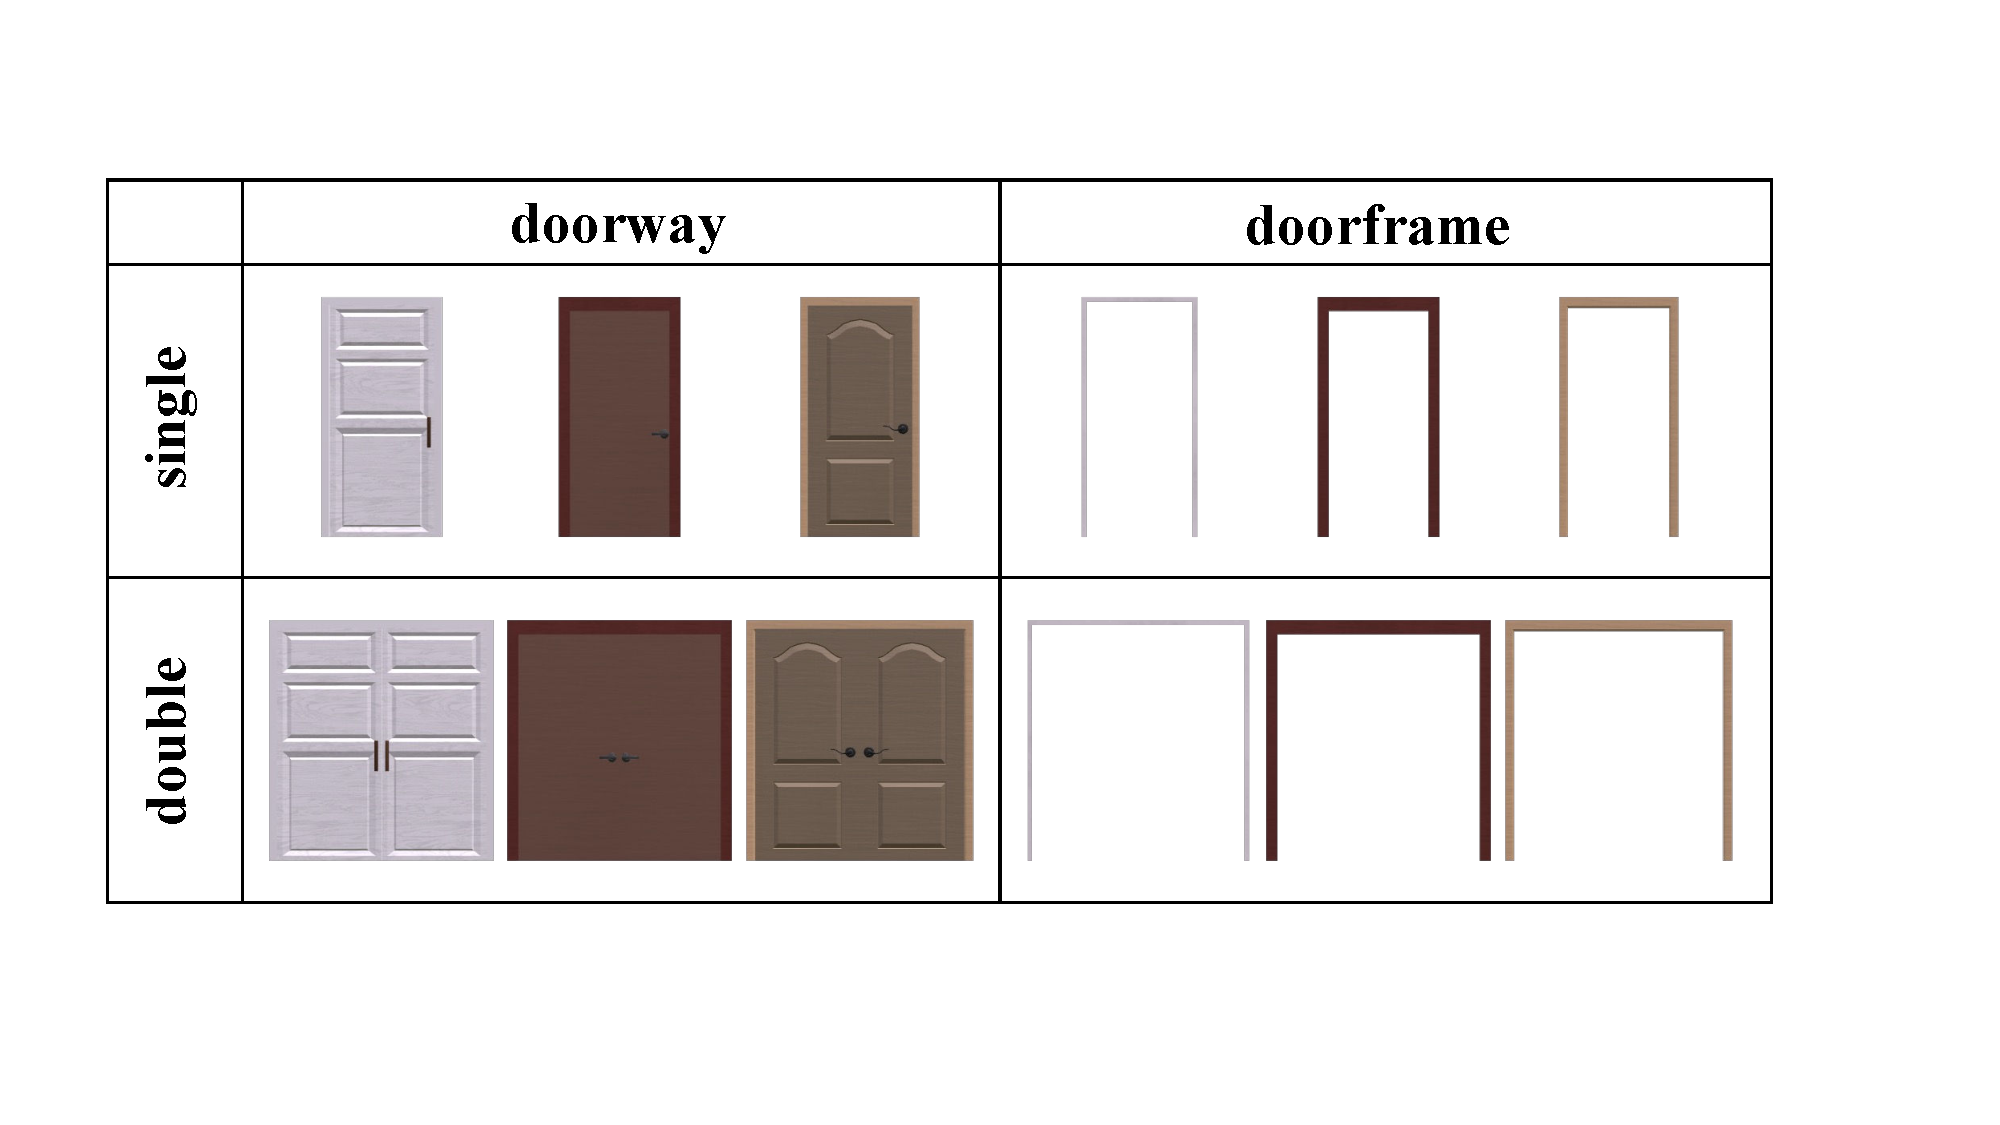
\includegraphics[width=8.3cm]{images/door.pdf}
    \caption{Examples of different doors in \holodeck.}
    \label{fig: door_assets}
    \vspace{-0.4cm}
\end{figure}

\begin{figure}[!t]
\centering
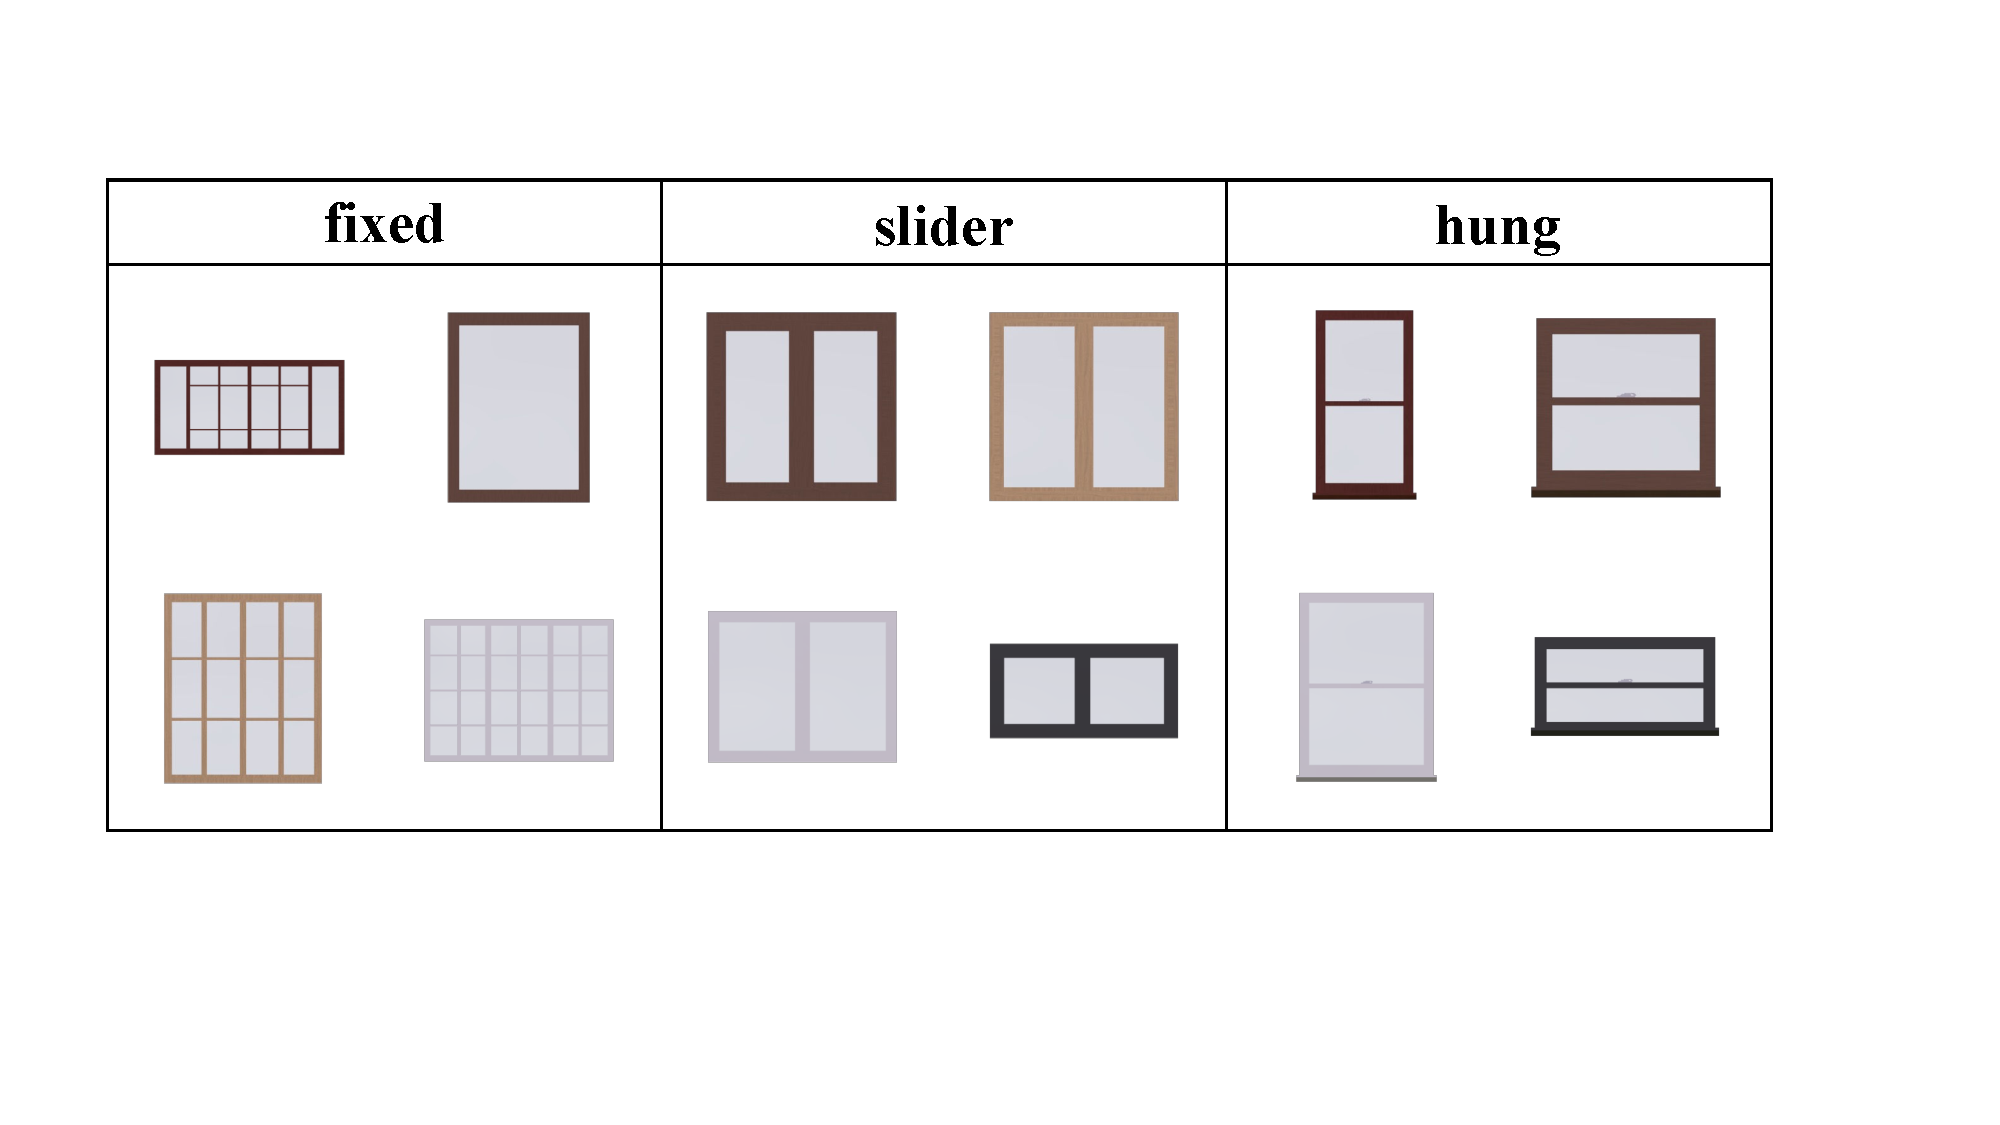
\includegraphics[width=8.3cm]{images/window.pdf}
    \caption{Examples of different windows in \holodeck.}
    \label{fig: window_assets}
    \vspace{-0.4cm}
\end{figure}

\begin{figure*}[!t]
\centering
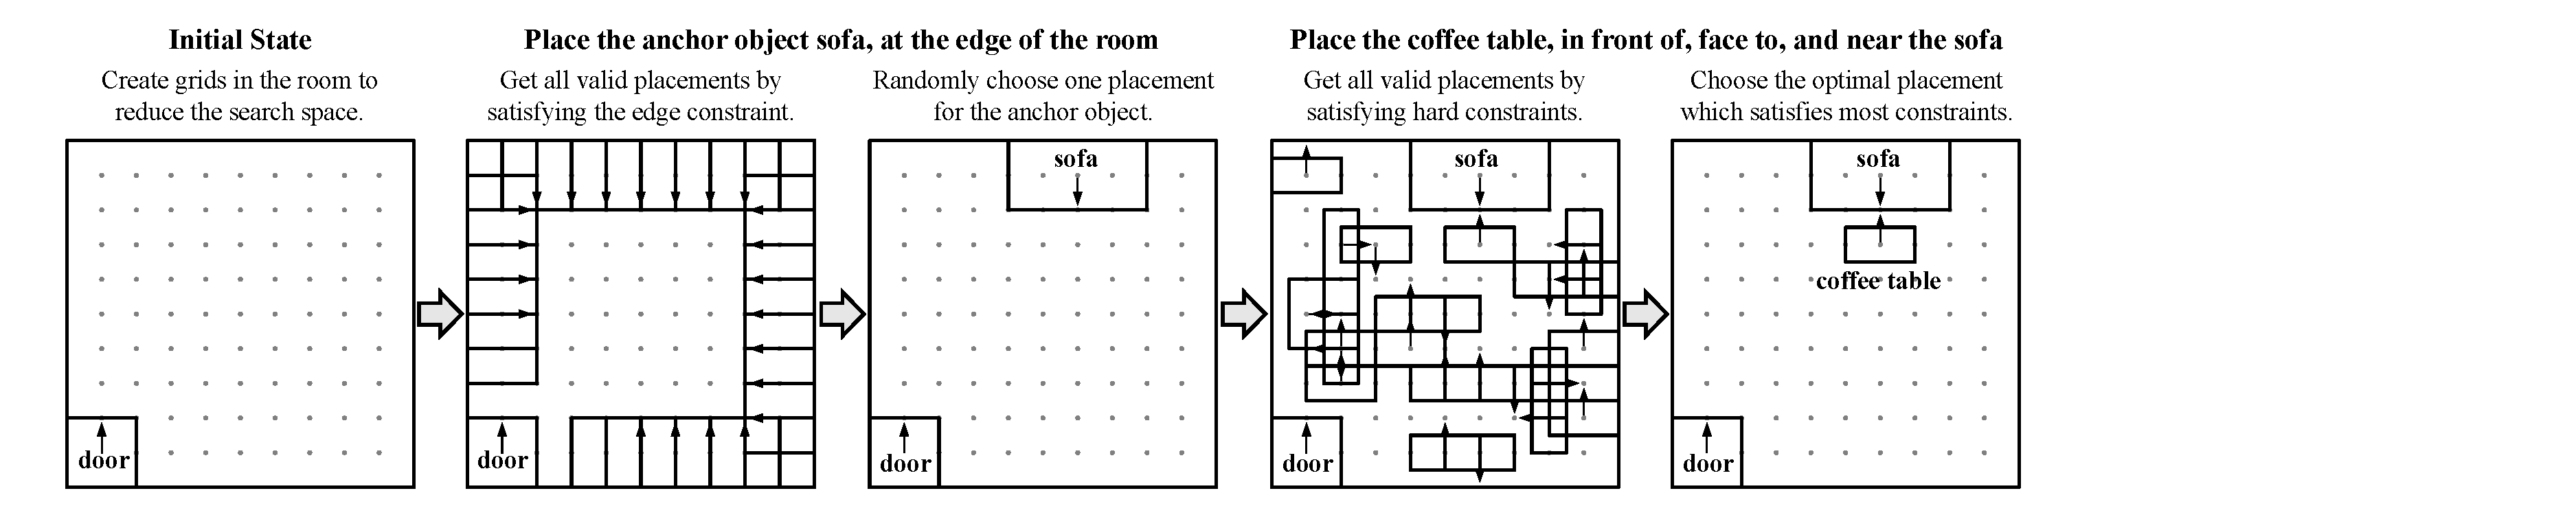
\includegraphics[width=\textwidth]{images/dfs.pdf}
    \caption{Example of using the DFS-based Constraint Satisfaction algorithm to place the objects.}
    \label{fig: dfs_demo}
    \vspace{-0.4cm}
\end{figure*}

\subsection{Object Selection Module} \label{sec: object selection module}

In Objaverse, each 3D asset $o \in \mathcal{O}$ is associated with the following metadata - a textual description of the asset $t$, the 3D bounding box size of the asset $\left(w, d, h\right)$, and a set of 2D images $I$ captured from three different angles ($0\degree$, $45\degree$, and $-45\degree$). 
For each object proposed by LLM $o'$, we have the LLM output a detailed description of the object ($t'$) and its 3D bounding box size $(w', d', h')$ for retrieval purposes.
%\begin{itemize}
    %\item \textbf{category}: the high-level category of the object, e.g., desk.
%    \item \textbf{description} ($t'$): a detailed description on the object.
%    \item \textbf{size} $(w', d', h')$: desired object dimensions (\textit{width}, \textit{depth}, \textit{height}).
    %\item \textbf{location}: on the floor or the wall.
    %\item \textbf{children objects}: the small objects on top of this object.
%\end{itemize}
%The LLM's proposed object $o'$ is characterized by $\left( t', \left(w', d', h'\right)\right)$. 
To evaluate the similarity between a candidate 3D asset in the repository $o = \left(t,  \left(w, d, h\right), I\right)$ and the object proposed by the LLM $o' \left( t', \left(w', d', h'\right)\right)$, we use three metrics:

\begin{itemize}
    \item \textbf{Visual Similarity} ($\mathcal{V}$) measures the CLIP similarity between the 2D renderings of the candidate asset and the textual description of the LLM-proposed object: $\mathcal{V}(o, o') = \max_{i \in I}\text{CLIP}(i, t')$.
    \item \textbf{Textual Similarity} ($\mathcal{T}$) measures the similarity between the textual description of the candidate 3D asset and the textural description of the LLM-proposed object. This metric is crucial in improving the accuracy of the retrieval process since it ensures that we retrieve the asset within the correct category. We use the sentence transformer (SBERT) \cite{reimers-2019-sentence-bert} with \href{https://huggingface.co/sentence-transformers/all-mpnet-base-v2}{all-mpnet-base-v2} checkpoint to calculate the scores: $\mathcal{T} = \text{SBERT}(t, t')$.
    %two assets with high visual similarity may belong to different categories, e.g., a blue sofa looks very close to a yoga mat. Textual similarity 
    \item \textbf{Size Discrepancy} ($\mathcal{S}$) measures the discrepancy in the size of the 3D bounding box size of the candidate asset and the LLM-proposed object. There are similar objects with different sizes in the asset repository, and the size of objects is an important factor in designing scenes, e.g., we need a larger sofa for a large living room. The size matching score is computed as: $\mathcal{S}(o, o') = \left(|w-w'| + |h - h'| + |d - d'|\right)/3$. Two objects of similar size will have a smaller value of $\mathcal{S}$.
\end{itemize}

The overall matching score $\mathcal{M} \left(o, o'\right)$ is a weighted sum of the above metrics:
\begin{equation}
    \mathcal{M} \left(o, o'\right) = \alpha \cdot \mathcal{V}\left(o, o'\right) + \beta \cdot \mathcal{T} (o, o') - \gamma \cdot \mathcal{S} (o, o')
\end{equation}
with weights $\alpha = 100$, $\beta = 1$, and $\gamma = 10$. The asset with the highest matching score is selected.

\subsection{Layout Design Module} \label{sec: object placement module}
In this module, we position the set of objects $O$ chosen in Sec \ref{sec: object selection module}, applying spatial relational constraints provided by the LLM. We define various constraints for floor objects:
\begin{itemize}
    \item \textbf{Global constraint}: edge; middle.
    \item \textbf{Distance constraint}: near (object); far (object).
    \item \textbf{Position constraint}: in front of (object); side of (object).
    \item \textbf{Alignment constraint}: center align with (object).
    \item \textbf{Direction constraint}: face to (object).
\end{itemize}

The LLM can combine these constraints to form a constraint list $C_o$ for each object $o \in O$. For instance, as shown in Figure \ref{fig: dfs_demo}, the constraints for a ``coffee table'' are [\text{middle}, \text{in front of (sofa)}, \text{face to (sofa)}, \text{near (sofa)}].

For floor object placement, we employ two solvers: Depth-First-Search (DFS) Solver and Mixed Integer Linear Programming (MILP) \cite{benichou1971experiments} Solver.
\smallbreak
\noindent \textbf{Depth-First-Search Solver.} In the DFS solver, each object is defined by five variables $\left(x, y, w, d, \text{rotation}\right)$. $\left(x, y\right)$ is the 2D coordinates of the object's center, $w$ and $d$ are the width and depth of the 2D bounding box of the object, and rotation can be one of 0°, 90°, 180°, and 270°.
The constraints listed above are treated softly, allowing certain violations when finding a layout.
% Each constraint can be verified using those three variables of objects, e.g., two objects are \textit{near} to each other if the distance between their 2D coordinates is small.
Beyond these soft constraints, we implement hard constraints essential for object placement: these constraints prevent object collisions and ensure that objects remain within the designated room boundaries. Violation of these hard constraints results in the object not being placed. Figure \ref{fig: dfs_demo} demonstrates that our DFS solver initiates grids to establish a finite search space. It first explores different placements for the anchor object selected by the LLM. Subsequent steps involve optimizing the placement for the remaining objects, adhering to the hard constraints, and satisfying as many soft constraints as possible.\footnote{The evaluation of an object's placement is based on the number of constraints satisfied. Placements that satisfy a greater number of constraints receive higher weights. However, any placement that violates hard constraints is rejected.} The algorithm can yield multiple solutions, with the final selection meeting the most constraints.
\smallbreak
\noindent \textbf{Mixed Integer Linear Programming (MILP) Solver} is particularly effective for structured layout design. It optimizes a linear objective function subject to linear constraints with some non-discrete variables. This approach is well-suited for our layout optimization problem in \holodeck.
% An integer linear programming problem is a mathematical optimization problem in which some or all variables are restricted to integers, and the objective function and the constraints (other than the integer constraints) are linear. If some decision variables are not discrete, the problem is known as a mixed-integer linear programming (MILP) problem. For our specific application, we utilize GUROBI~\cite{gurobi}, a state-of-the-art optimization solver renowned for its efficiency and robustness in handling MILP problems.
% An integer linear programming problem optimizes a linear objective function under linear constraints, with variables either entirely or partially restricted to integers. In mixed-integer linear programming (MILP), some variables remain non-discrete, suitable for structured layout design.

% Each object's position is defined by four variables ($x$, $y$, $
% \text{rotate}_{90}$, $\text{rotate}_{180}$), where $\text{rotate}_{90}$ is a boolean variable that indicates whether the object is rotated by 90 degrees and $\text{rotate}_{180}$ is also a boolean variable that indicates whether the object is rotated by 180 degrees. For example, if both $
% \text{rotate}_{90}$ and $\text{rotate}_{180}$ are true, this configuration represents a 270-degree rotation (90 + 180 degrees) of the object.
In our MILP formulation, each object's position is determined by four variables: ($x$, $y$, $\text{rotate}_{90}$, $\text{rotate}_{180}$). The variables $\text{rotate}_{90}$ and $\text{rotate}_{180}$ are boolean, indicating rotations of 90 and 180 degrees, respectively. For example, if $\text{rotate}_{90}$ and $\text{rotate}_{180}$ are both true, it signifies a 270-degree rotation of the object.
We translate all previously mentioned constraints into linear ones for the MILP problem. For instance, to align Object A with Object B at the center, a constraint in the form of \(A_x = B_x\) or \(A_y = B_y\) is implemented, where \(A_x, A_y\) and \(B_x, B_y\) represent the centers of Objects A and B, respectively. Note that the constraint is non-linear due to the OR operator. To model this linearly in MILP, we can introduce binary auxiliary variables and additional constraints to capture the logic of the OR condition.
For solving the MILP, we utilize GUROBI \cite{gurobi}, a state-of-the-art solver known for its efficiency and robustness. 

In MILP solver, all constraints specified in the previous section are applied as hard constraints except that the Distance constraints (\textit{near} and \textit{far}) are uniquely modeled as part of the objective. For a visual comparison of these solvers' outcomes in \holodeck, refer to Figure~\ref{fig: layout}.
\smallbreak
\noindent \textbf{Wall \& Small Objects.} The placement of wall objects is determined by two specific attributes:
\begin{itemize}
\item \textbf{Above (Floor Object)}: This denotes the floor object directly underneath the wall object.
\item \textbf{Height}: Specifies the exact distance from the floor to the base of the wall object, measured in centimeters.
\end{itemize}

To place small surface objects on top of larger objects, we first have LLM propose the placements and utilize\texttt{RandomSpawn}\footnote{\href{https://ai2thor.allenai.org/ithor/documentation/objects/domain-randomization/\#initial-random-spawn}{AI2-THOR RandomSpawn Documentation}} function in AI2-THOR. This method allows for randomized and efficient positioning of small objects on larger surfaces.

\begin{figure}[!t]
\centering
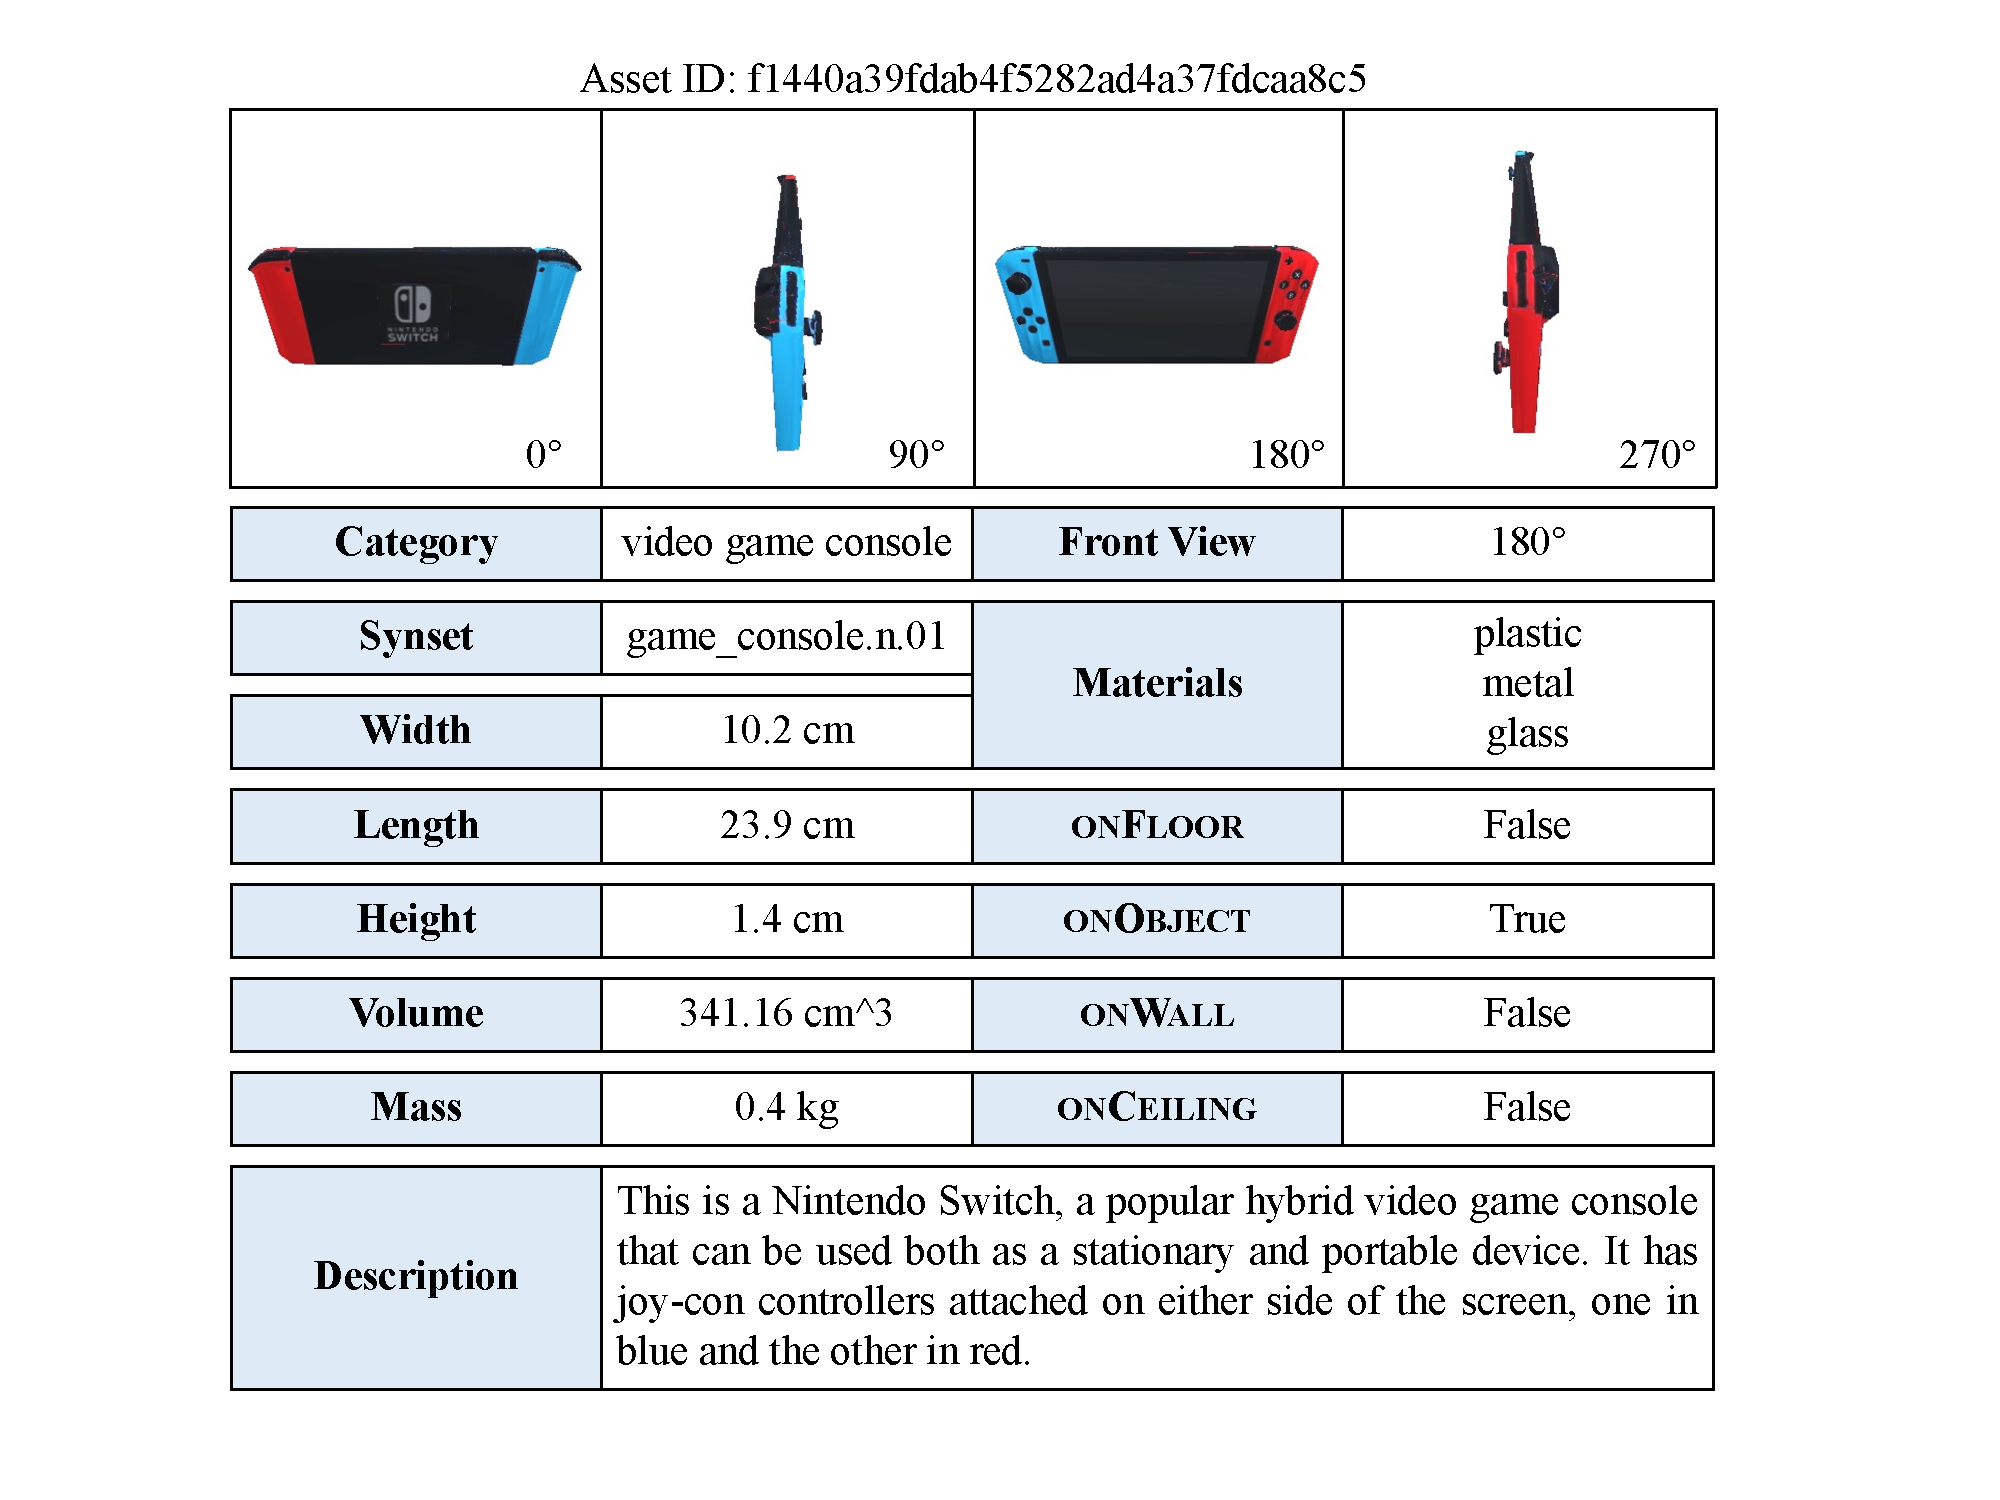
\includegraphics[width=8.3cm]{images/asset_annotation.pdf}
    \caption{Example of an asset's attributes annotated by GPT-4-V.}
    \label{fig: asset_annotation}
    \vspace{-0.4cm}
\end{figure}

\subsection{GPT-4-V for 3D Asset Annotation}
We annotate the 3D assets used in \holodeck with OpenAI's \href{https://openai.com/research/gpt-4v-system-card}{GPT-4-V API} 
to enhance the accuracy of object retrieval and placement. As illustrated in Figure \ref{fig: asset_annotation}, GPT-4-V takes a set of four images as inputs, each showing an object from orthogonal rotations (0°, 90°, 180°, and 270°) and outputs the following attributes for the 3D object:
\begin{itemize}
\item \textbf{Category}: a specific classification of the object, such as ``chair'', ``table'', ``building'', etc.
\item \textbf{Synset}: the nearest WordNet \cite{miller1995wordnet} synset will be used as the object type in object navigation tasks.
\item \textbf{Width, Length, Height}: physical dimensions in centimeters, defining the object's bounding box sizes.
\item \textbf{Volume}: approximate volume in cubic centimeters (cm$^3$).
\item \textbf{Mass}: estimated object mass in kilograms (kg).
\item \textbf{Front View}: an integer denoting the view representing the front of the object, often the most symmetrical view.
\item \textbf{Description}: a detailed textual description of the object.
\item \textbf{Materials}: a list of materials constituting the object.
\item \textbf{Placement Attributes:} Boolean values (\textsc{onCeiling}, \textsc{onWall}, \textsc{onFloor}, \textsc{onObject}) indicating typical placement locations. For example, ``True'' for a ceiling fan's placement on the ceiling.
\end{itemize}

\subsection{Importing Objaverse Assets into AI2-THOR} \label{appendix: objaverse assets}
The transformation of Objaverse assets into interactive objects in AI2-THOR involves a complex, multi-step pipeline.

Initially, the process starts with downloading and converting various 3D models into a mesh format optimized for runtime loading.
We then generate visibility points on the mesh surface, enabling AI2-THOR to determine object visibility.
This is followed by 3D decomposition, where the mesh is split into simpler convex meshes to facilitate rapid and realistic collision detection.
The final step involves compressing textures (i.e., albedo, normal, and emission) and the model format to streamline performance.

Handling many assets in numerous scenes is challenging, mainly due to the large mesh counts of Objaverse assets and the traditional compile-time asset packaging approach of game engines like Unity. To address this, we implement caching layers for objects, reducing the loading time for repeated use in different scenes. Additionally, we develop a system to unload objects from memory, allowing efficient management of thousands of 3D objects at runtime.

Besides the objects from Objaverse, our automated pipeline can process any 3D objects, including those generated by text-to-3D models, as shown in Figure \ref{fig: add new asset}.

\subsection{Rendering Options}
As shown in Figure \ref{fig: unity_vs_blender}, \holodeck scenes are rendered by Unity as default to train the embodied agents more efficiently. Users can also render \holodeck scenes in Blender to achieve better realism.

\begin{figure}[!t]
\centering
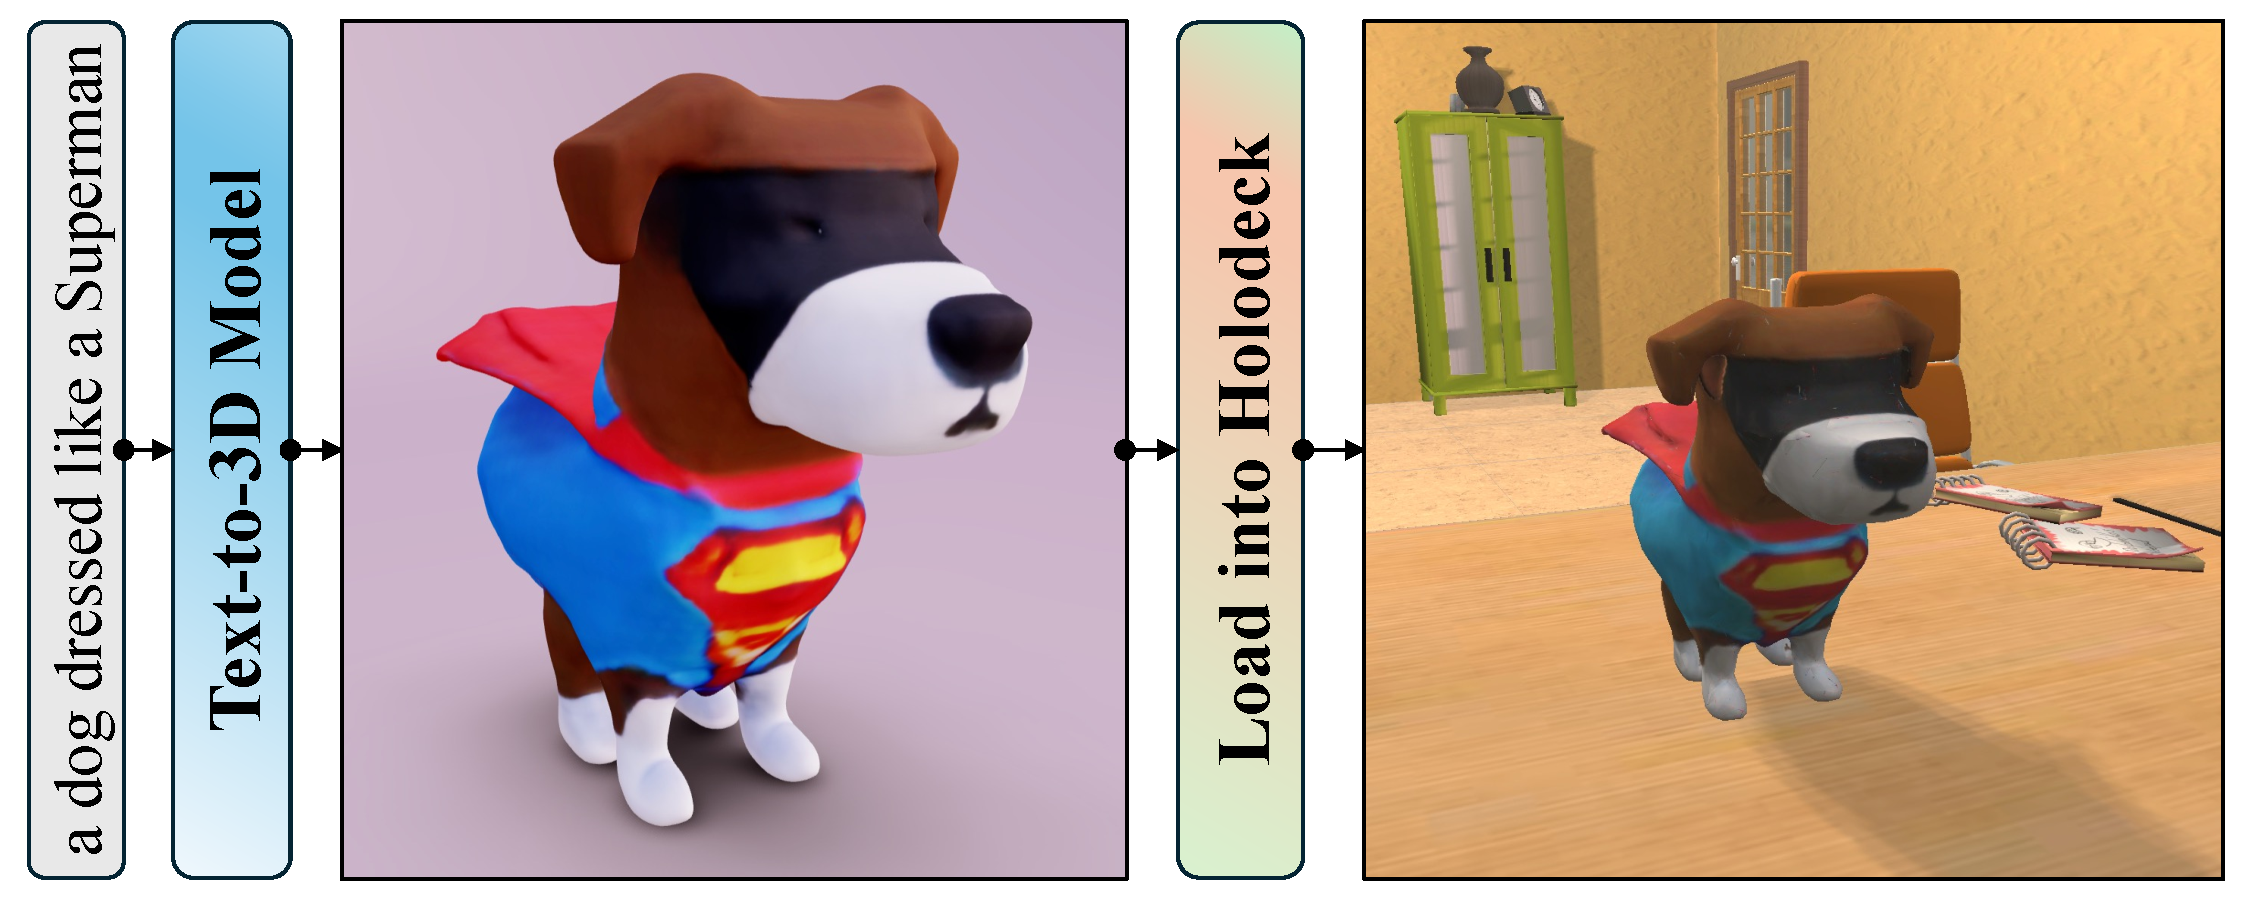
\includegraphics[width=8.3cm]{images/add_new_asset.pdf}
    \caption{\holodeck can import any 3D objects, including text-to-3D models generated (e.g., the object in this figure is generated by LumaAI \cite{luma2023}) to enhance object diversity.}
    \label{fig: add new asset}
    \vspace{-0.4cm}
\end{figure}

\subsection{Prompt} \label{appendix: prompt}
The complete prompt templates of \holodeck's modules are provided in Figure \ref{fig:prompt-1} and \ref{fig:prompt-2}. The prompt for annotating 3D assets using GPT-4-V is shown in Figure \ref{fig:prompt-3}.

\begin{figure}[!t]
\centering
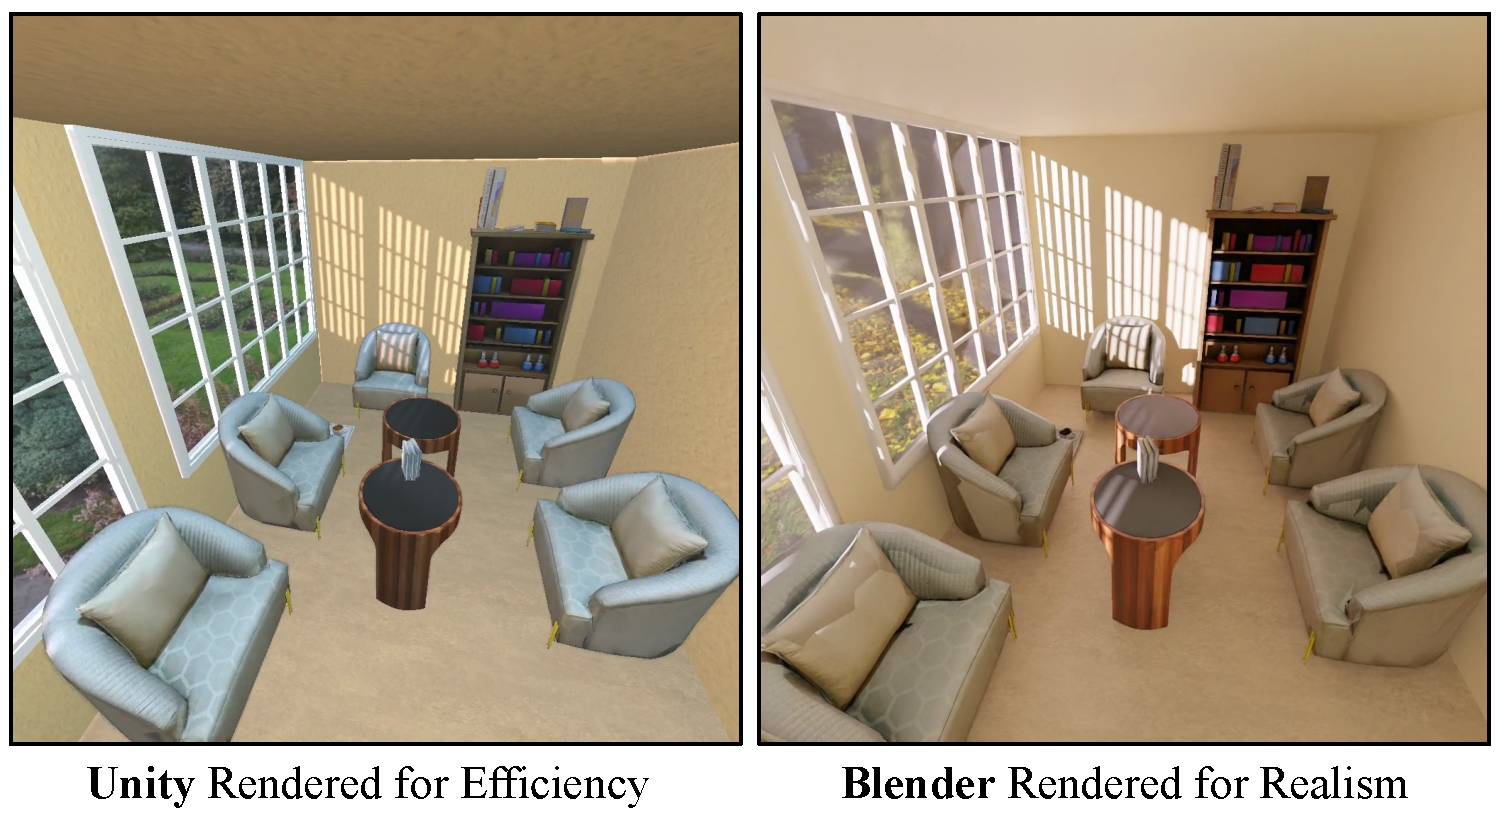
\includegraphics[width=8.3cm]{images/unity_vs_blender.pdf}
    \caption{\holodeck renders scenes with Unity by default for efficiency to facilitate Embodied AI applications. Blender can also be used to render \holodeck scenes to improve realism.}
    \label{fig: unity_vs_blender}
\end{figure}

\section{Qualitative Examples}
In Figure \ref{fig: mit_scenes_add}, we showcase an additional 20 scenes generated by \holodeck. These 20 scene types are chosen from the MIT dataset \cite{quattoni2009recognizing}, distinct from examples in the main paper. Figure \ref{fig: layout} presents a comparative analysis of layouts created by five methods. Figure \ref{fig: system_compare} offers a visual comparison of residential scenes from iTHOR, \procthor, and \holodeck, highlighting the differences and capabilities of each system.

\section{\noveltythor}
\noveltythor comprises human-designed scenes crafted to challenge embodied agents in unique and diverse environments with a wide array of assets from Objaverse.

To integrate Objaverse assets into Unity, we developed tools that run a conversion pipeline on various operating systems, including macOS and Windows. This flexibility also enables the inclusion of assets other than those found in Objaverse. We designed a user-friendly interface for our artists and designers, facilitating asynchronous asset integration while optimizing storage efficiency.

The critical step of this process is the generation of Unity templates (prefabs) for the assets and their associated resources, leading to the creation of the scenes discussed in this paper. Figures \ref{fig: noveltythor} and \ref{fig: noveltythor_continued} showcase top-down views of the 10 \noveltythor scenes, spanning five categories. 
% The development of these scenes took approximately 20 working days for two 3D artists.

\begin{figure}[!t]
\centering
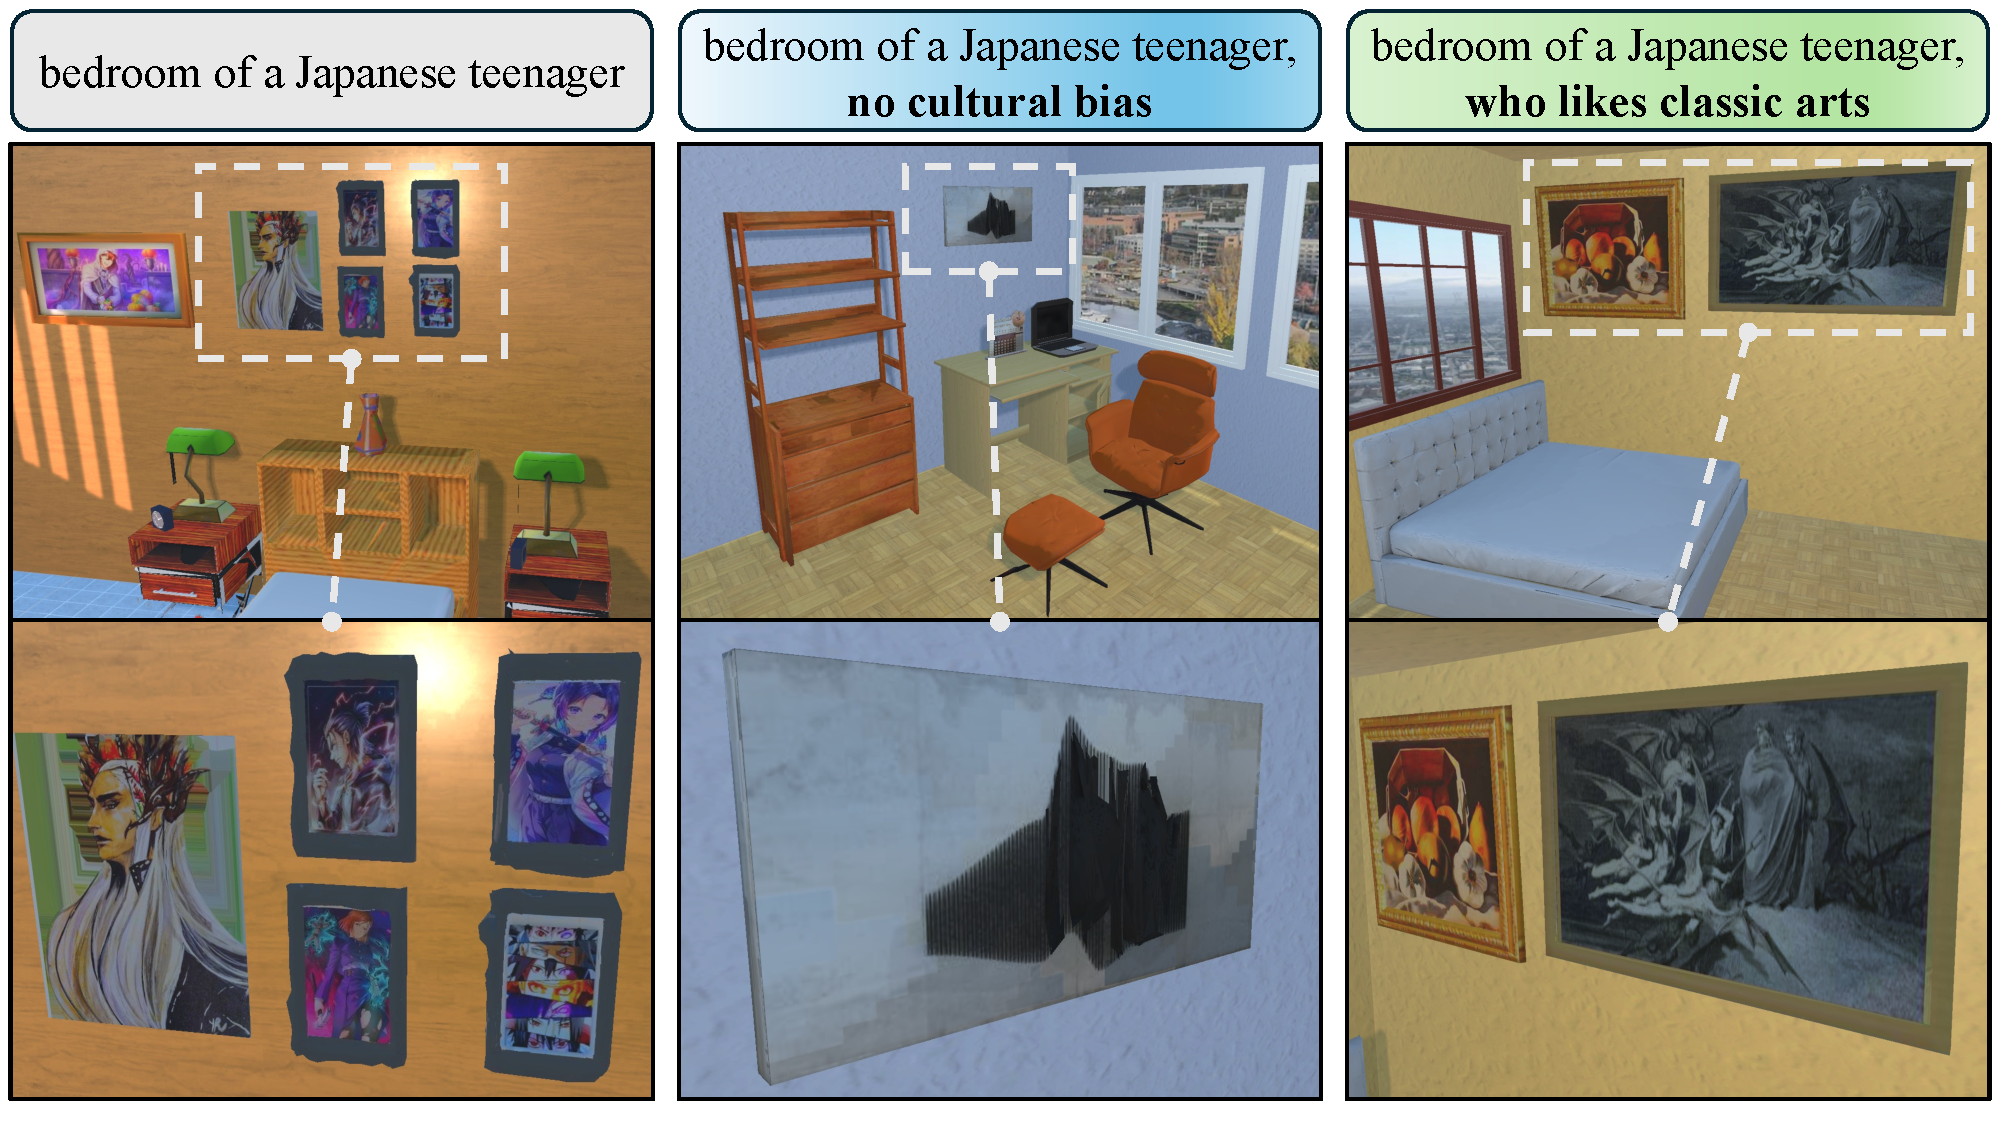
\includegraphics[width=8.3cm]{images/mitigate_bias.pdf}
    \caption{We can address the cultural bias of GPT-4 by prompting.}
    \label{fig: mitigate bias}
    \vspace{-0.4cm}
\end{figure}

\section{Cultural Bias}
Cultural biases in \holodeck generation can stem from biases in the LLM and the 3D asset retrieval component. For example, in Figure \ref{fig: mitigate bias} (left), when the prompt contains culturally specific terms such as ``Japanese'', the generated scene may disproportionately feature prototypical objects like Manga posters. One mitigation strategy is to adjust the prompts, e.g., users can control the generation by simply adding a suffix like ``no cultural bias'' or making the prompt more detailed. This strategy is unlikely to fully remove bias, but these qualitative results suggest it can significantly help.

\begin{figure*}[!b]
    \centering
    \begin{center}
    
    \begin{tcolorbox} [top=2pt,bottom=2pt, width=\linewidth, boxrule=1pt]
    {\footnotesize {\fontfamily{zi4}\selectfont
    \textbf{Floor plan Prompt:}
    You are an experienced room designer. Please assist me in crafting a floor plan. Each room is a rectangle. You need to define the four coordinates and specify an appropriate design scheme, including each room's color, material, and texture.
    Assume the wall thickness is zero. Please ensure that all rooms are connected, not overlapped, and do not contain each other. The output should be in the following format: room name | floor material | wall material | vertices (coordinates). Note: the units for the coordinates are meters. \\
    For example: \\
    living room | maple hardwood, matte | light grey drywall, smooth | [(0, 0), (0, 8), (5, 8), (5, 0)]\\
    kitchen | white hex tile, glossy | light grey drywall, smooth | [(5, 0), (5, 5), (8, 5), (8, 0)] \\
    
    Here are some guidelines for you: \\
    1. A room's size range (length or width) is 3m to 8m. The maximum area of a room is 48 m$^2$. Please provide a floor plan within this range and ensure the room is not too small or too large. \\
    2. It is okay to have one room in the floor plan if you think it is reasonable. \\
    3. The room name should be unique. \\
    
    Now, I need a design for \{input\}. \\
    Additional requirements: \{additional\_requirements\}. \\
    
    Your response should be direct and without additional text at the beginning or end.
    }
    \par}
    \end{tcolorbox}

    \begin{tcolorbox} [top=2pt,bottom=2pt, width=\linewidth, boxrule=1pt]
    {\footnotesize {\fontfamily{zi4}\selectfont
    \textbf{Wall Height Prompt:}
    I am now designing \{input\}. Please help me decide the wall height in meters.
    Answer with a number, for example, 3.0. Do not add additional text at the beginning or in the end.
    }
    \par}
    \end{tcolorbox}

    \begin{tcolorbox} [top=2pt,bottom=2pt, width=\linewidth, boxrule=1pt]
    {\footnotesize {\fontfamily{zi4}\selectfont
    \textbf{Doorway Prompt:}
    I need assistance in designing the connections between rooms. The connections could be of three types: doorframe (no door installed), doorway (with a door), or open (no wall separating rooms). The sizes available for doorframes and doorways are single (1m wide) and double (2m wide). \\
    
    Ensure that the door style complements the design of the room. The output format should be: room 1 | room 2 | connection type | size | door style.
    For example: \\
    exterior | living room | doorway | double | dark brown metal door \\
    living room | kitchen | open | N/A | N/A \\
    living room | bedroom | doorway | single | wooden door with white frames \\
    
    The design under consideration is \{input\}, which includes these rooms: \{rooms\}. \\
    The length, width, and height of each room in meters are:
    \{room\_sizes\} \\
    Certain pairs of rooms share a wall: \{room\_pairs\}. There must be a door to the exterior. \\
    Adhere to these additional requirements \{additional\_requirements\}. \\
    
    Provide your response succinctly, without additional text at the beginning or end.
    }
    \par}
    \end{tcolorbox}

    \begin{tcolorbox} [top=2pt,bottom=2pt, width=\linewidth, boxrule=1pt]
    {\footnotesize {\fontfamily{zi4}\selectfont
    \textbf{Window Prompt:}
    Guide me in designing the windows for each room. The window types are: fixed, hung, and slider. \\
    The available sizes (width x height in cm) are: \\
    fixed: (92, 120), (150, 92), (150, 120), (150, 180), (240, 120), (240, 180) \\
    hung: (87, 160), (96, 91), (120, 160), (130, 67), (130, 87), (130, 130) \\
    slider: (91, 92), (120, 61), (120, 91), (120, 120), (150, 92), (150, 120) \\
    
    Your task is to determine the appropriate type, size, and quantity of windows for each room, bearing in mind the room's design, dimensions, and function.
    
    Please format your suggestions as follows: room | wall direction | window type | size | quantity | window base height (cm from floor). For example:
    living room | west | fixed | (130, 130) | 1 | 50 \\
    
    I am now designing \{input\}. The wall height is \{wall\_height\} cm. \\
    The walls available for window installation (direction, width in cm) in each room are:
    \{walls\} \\
    Please note: It is not mandatory to install windows on every available wall. Within the same room, all windows must be the same type and size.
    Also, adhere to these additional requirements: \{additional\_requirements\}. \\
    
    Provide a concise response, omitting any additional text at the beginning or end. 
    }
    \par}
    \end{tcolorbox}
    
    \end{center}
    \caption{Prompt templates for Floor Module, Wall Module, Doorway Module, and Window Module.}
    \label{fig:prompt-1}
    \vspace{-.3cm}
\end{figure*}
\begin{figure*}[!t]
    \centering
    \begin{center}
    
    \begin{tcolorbox} [top=2pt,bottom=2pt, width=\linewidth, boxrule=1pt]
    {\footnotesize {\fontfamily{zi4}\selectfont
    \textbf{Object Selection Prompt:}
    You are an experienced room designer, please assist me in selecting large *floor*/*wall* objects and small objects on top of them to furnish the room. You need to select appropriate objects to satisfy the customer's requirements.
    You must provide a description and desired size for each object since I will use it to retrieve objects. If multiple identical items are to be placed in the room, please indicate the quantity and variance type (same or varied).
    Present your recommendations in JSON format:

    \{ 
        object\_name:\{ \\
            "description": a short sentence describing the object, \\
            "location": "floor" or "wall", \\
            "size": the desired size of the object, in the format of a list of three numbers, [length, width, height] in centimeters, \\
            "quantity": the number of objects (int), \\
            "variance\_type": "same" or "varied", \\
            "objects\_on\_top": a list of small children objects (can be empty) which are placed *on top of* this object. For each child object, you only need to provide the object\ name, quantity and variance type. For example, \{"object\_name": "book", "quantity": 2, "variance\_type": "varied"\}
        \}
    \} \\
    
    *ONE-SHOT EXAMPLE* \\
    
    Currently, the design in progress is *INPUT*, and we are working on the *ROOM\_TYPE* with the size of ROOM\_SIZE.
    Please also consider the following additional requirements: REQUIREMENTS.
    
    Here are some guidelines for you: \\
    1. Provide reasonable type/style/quantity of objects for each room based on the room size to make the room not too crowded or empty. \\
    2. Do not provide rug/mat, windows, doors, curtains, and ceiling objects which have been installed for each room. \\
    3. I want at least 10 types of large objects and more types of small objects on top of the large objects to make the room look more vivid. \\
    
    Please first use natural language to explain your high-level design strategy for *ROOM\_TYPE*, and then follow the desired JSON format *strictly* (do not add any additional text at the beginning or end).
    }
    \par}
    \end{tcolorbox}

    \begin{tcolorbox} [top=2pt,bottom=2pt, width=\linewidth, boxrule=1pt]
    {\footnotesize {\fontfamily{zi4}\selectfont
    \textbf{Layout Design Prompt:}
    You are an experienced room designer.
    Please help me arrange objects in the room by assigning constraints to each object.
    Here are the constraints and their definitions: \\
    1. global constraint: \\
        1) edge: at the edge of the room, close to the wall, most of the objects are placed here. \\
        2) middle: not close to the edge of the room.
    
    2. distance constraint: \\
        1) near, object: near to the other object, but with some distanbce, 50cm < distance < 150cm. \\
        2) far, object: far away from the other object, distance >= 150cm.

    3. position constraint: \\
        1) in front of, object: in front of another object. \\
        2) side of, object: on the side (left or right) of another object.
    
    4. alignment constraint:
        1) center aligned, object: align the center of the object with the center of another object.
    
    5. Rotation constraint:
        1) face to, object: face to the center of another object. \\
    
    For each object, you must have one global constraint and you can select various numbers of constraints and any combinations of them and the output format must be:
    object | global constraint | constraint 1 | constraint 2 | ...
    
    For example:
    sofa-0 | edge \\
    coffee table-0 | middle | near, sofa-0 | in front of, sofa-0 | center aligned, sofa-0 | face to, sofa-0 \\
    tv stand-0 | edge | far, coffee table-0 | in front of, coffee table-0 | center aligned, coffee table-0 | face to, coffee table-0 \\
    
    Here are some guidelines for you: \\
    1. I will use your guideline to arrange the objects *iteratively*, so please start with an anchor object which doesn't depend on the other objects (with only one global constraint). \\
    2. Place the larger objects first. \\
    3. The latter objects could only depend on the former objects. \\
    4. The objects of the *same type* are usually *aligned*. \\
    5. I prefer objects to be placed at the edge (the most important constraint) of the room if possible which makes the room look more spacious. \\
    6. Chairs must be placed near to the table/desk and face to the table/desk. \\
    Now I want you to design \{room\_type\} and the room size is \{room\_size\}. \\
    Here are the objects that I want to place in the \{room\_type\}:
    \{objects\} \\
    Please first use natural language to explain your high-level design strategy, and then follow the desired format *strictly* (do not add any additional text at the beginning or end) to provide the constraints for each object.
    }
    \par}
    \end{tcolorbox}
    
    \end{center}
    \caption{Prompt templates for Object Selection Module and Layout Design Module.}
    \label{fig:prompt-2}
    \vspace{-.3cm}
\end{figure*}




\begin{figure*}[!t]
    \centering
    \begin{center}
        % Images
         % \textbf{3D Asset annotation Sample Prompt:} \\
    % 
\includegraphics[width=0.24\linewidth]{images/0.png} % Image 1
    % \hfill % This adds space between the images
    % \includegraphics[width=0.24\linewidth]{images/90.png} % Image 2
    % \hfill % Space
    % \includegraphics[width=0.24\linewidth]{images/180.png} % Image 3
    % \hfill % Space
    % \includegraphics[width=0.24\linewidth]{images/270.png} % Image 4
    % \vspace{-5mm}
    \begin{tcolorbox} [top=2pt,bottom=2pt, width=\linewidth, boxrule=1pt]
    {\footnotesize {\fontfamily{zi4}\selectfont
    \textbf{3D Asset annotation Prompt:}
   Please annotate this 3D asset with the following values (output valid JSON): \\
        "annotations": \{ \\
            "category": a category such as "chair", "table", "building", "person", "airplane", "car", "seashell", "fish", etc. Try to be more specific than "furniture", \\
            "synset": the synset of the object that is most closely related. This could be "cat.n.01", "glass.n.03", "bank.n.02", \\
            "width": approximate width in cm. For a human being, this could be "45", \\
            "length": approximate length in cm. For a human being, this could be "25", \\
            "height": approximate height in cm. For a human being, this could be "182", \\
            "volume": approximate volume in cm$^3$. For a human being, this could be "62000", \\
            "mass": approximate mass in kilogram. For a human being, this could be "72", \\
            "frontView": which of the views represents the front of the object (value should be an integer with the first image being 0). Note that the front view of an object, including furniture, tends to be the view that exhibits the highest degree of symmetry, \\
            "description": a description of the object (don't use the term "3D asset" here), \\
            "materials": a Python list of the materials that the object appears to be made of (roughly in order of most used material to least used), \\
            "onCeiling": whether this object can appear on the ceiling or not, return true or false with no explanations. This would be true for a ceiling fan but false for a chair, \\
            "onWall": whether this object can appear on the wall or not, return true or false with no explanations. This would be true for a painting but false for a table, \\
            "onFloor": whether this object can appear on the floor or not, return true or false with no explanations. This would be true for a piano but false for a curtain, \\
            "onObject": whether this object can appear on another object or not, return true or false with no explanations. This would be true for a laptop but not for a sofa
        \} \\ \\
Please output the JSON now.
}
    \par}
    \end{tcolorbox}

    \end{center}
    \caption{Prompt template for annotating 3D assets with GPT-4-V.}
    \label{fig:prompt-3}
    %\vspace{-.3cm}
\end{figure*}






\begin{figure*}[!b]
\centering
\includegraphics[width=\textwidth]{images/mit_scenes_1.pdf}
    \caption{Additional examples of different scene types from MIT Scenes \cite{quattoni2009recognizing}.}
    \label{fig: mit_scenes_add}
\end{figure*}


\begin{figure*}[!t]
\centering
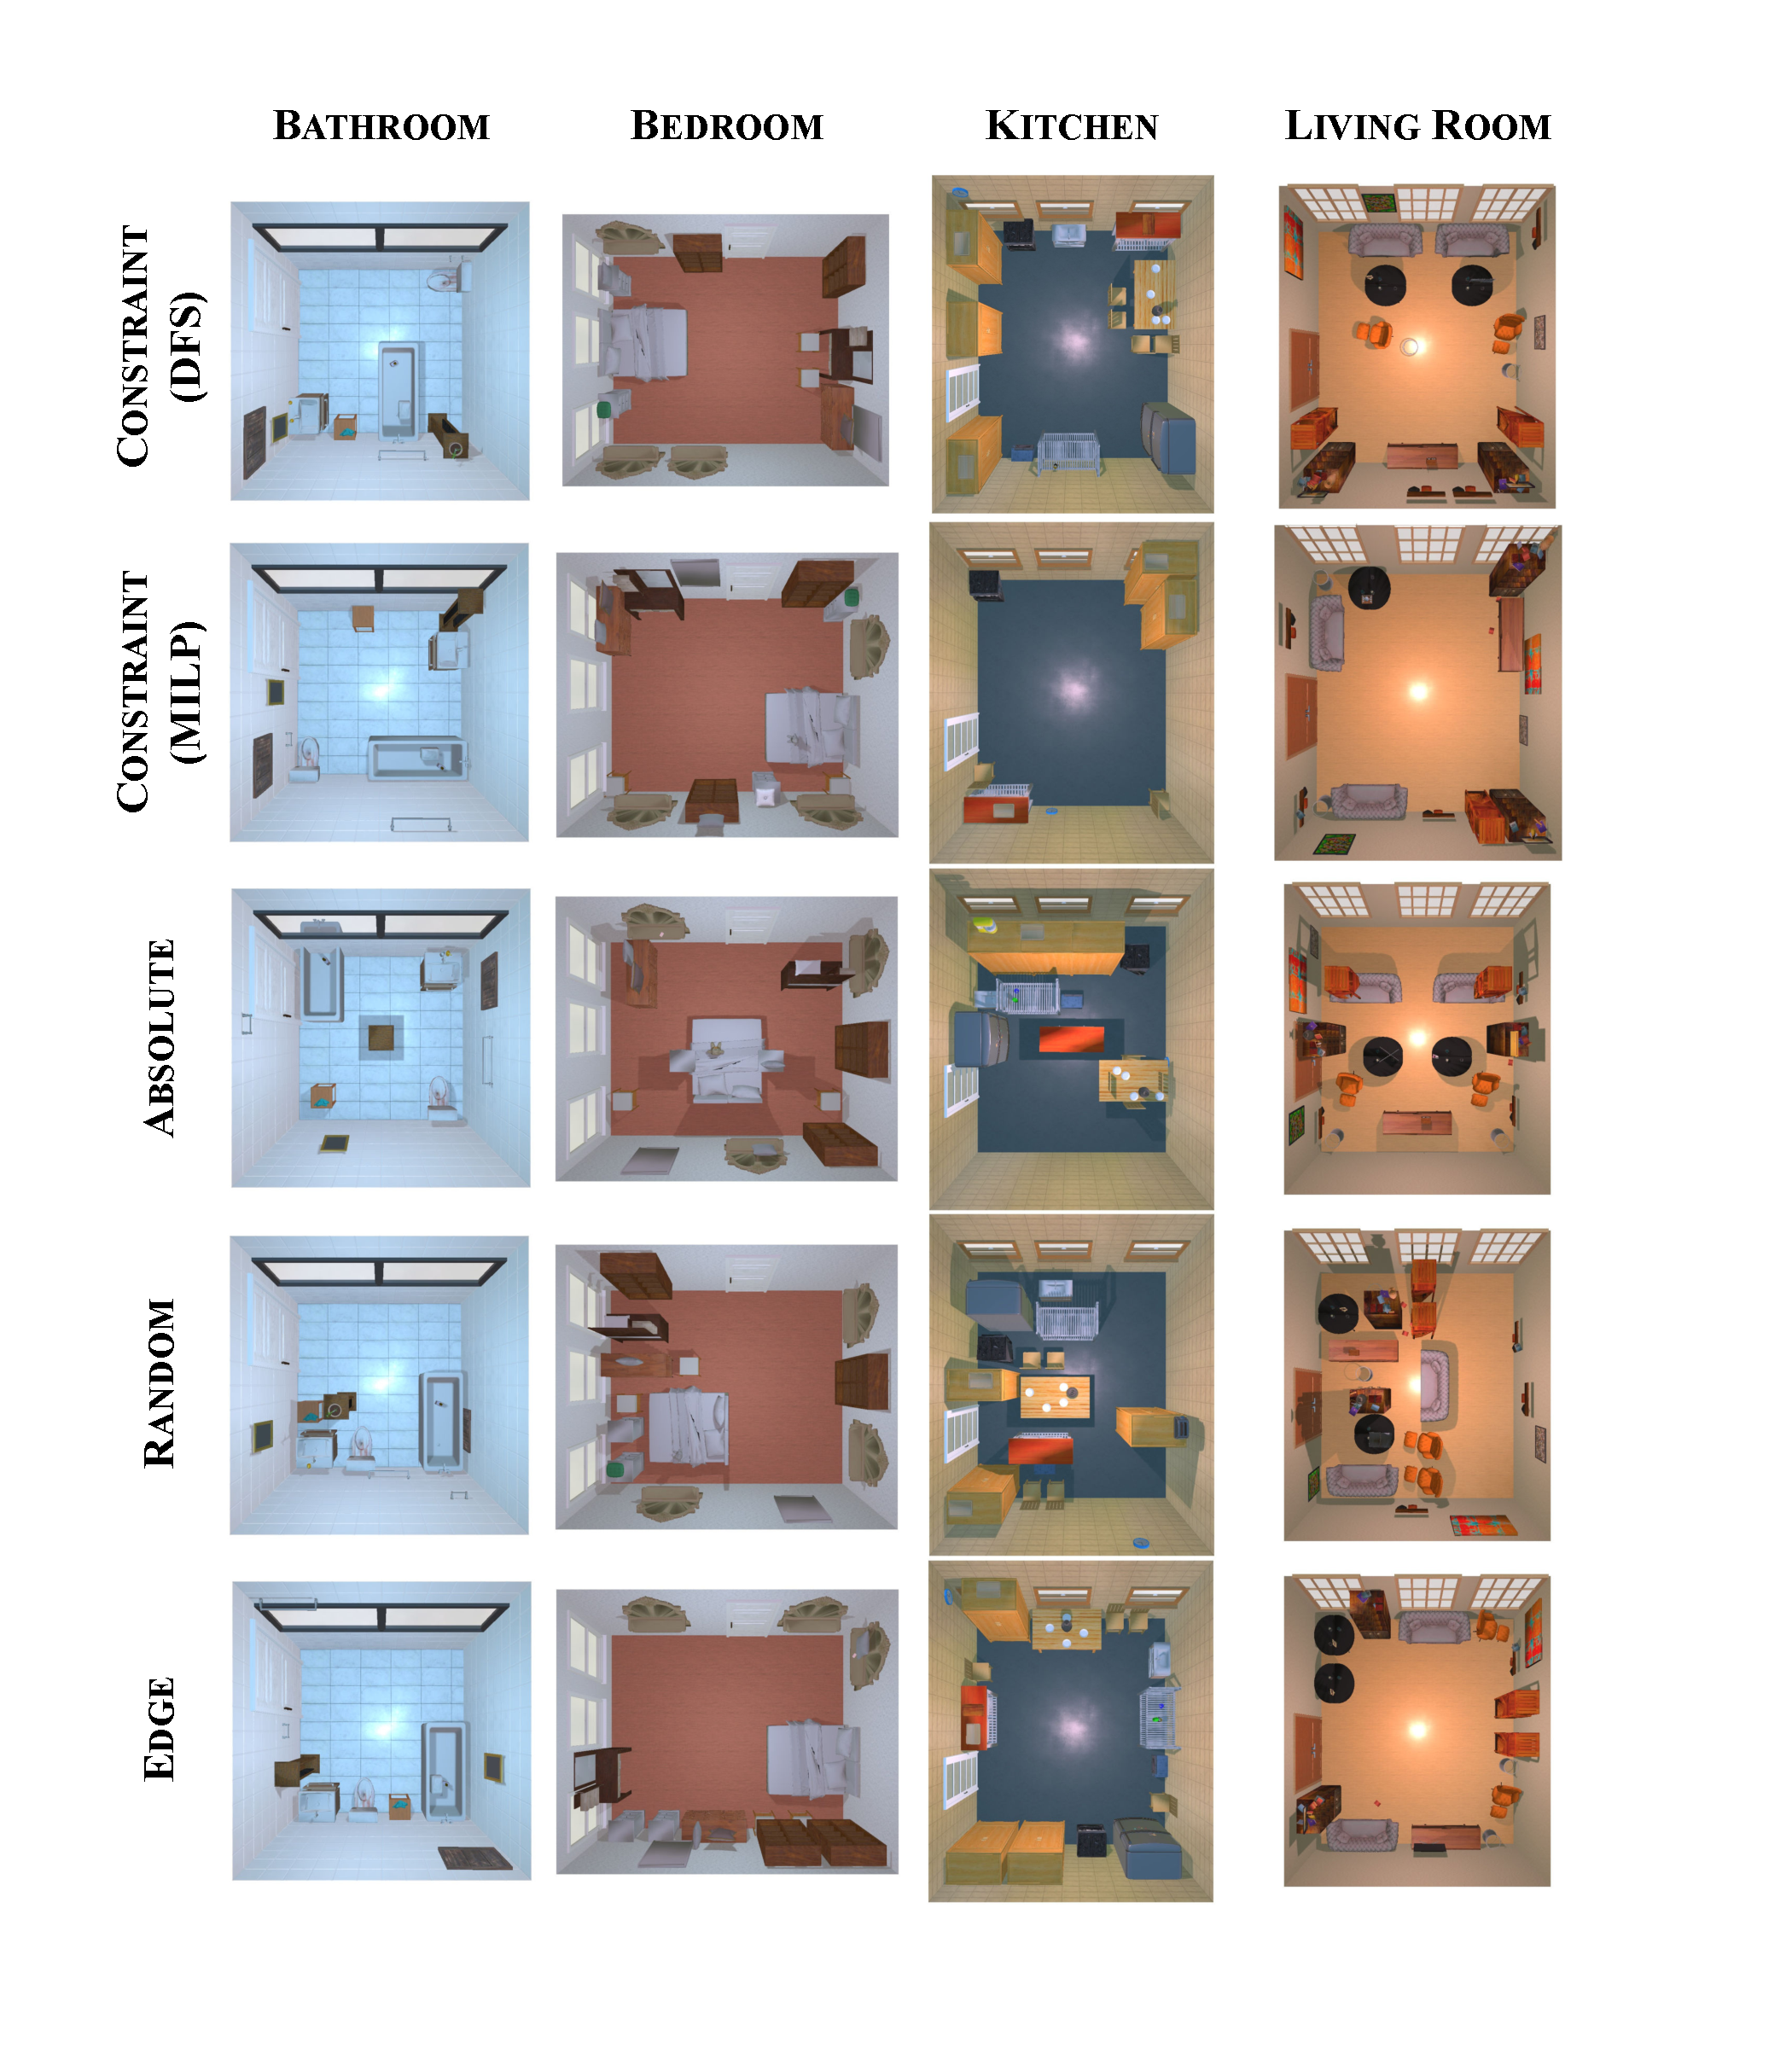
\includegraphics[width=17cm]{images/layout_compare.pdf}
    \caption{Qualitative comparison of the different layout methods.}
    \label{fig: layout}
\end{figure*}

\begin{figure*}[!t]
\centering
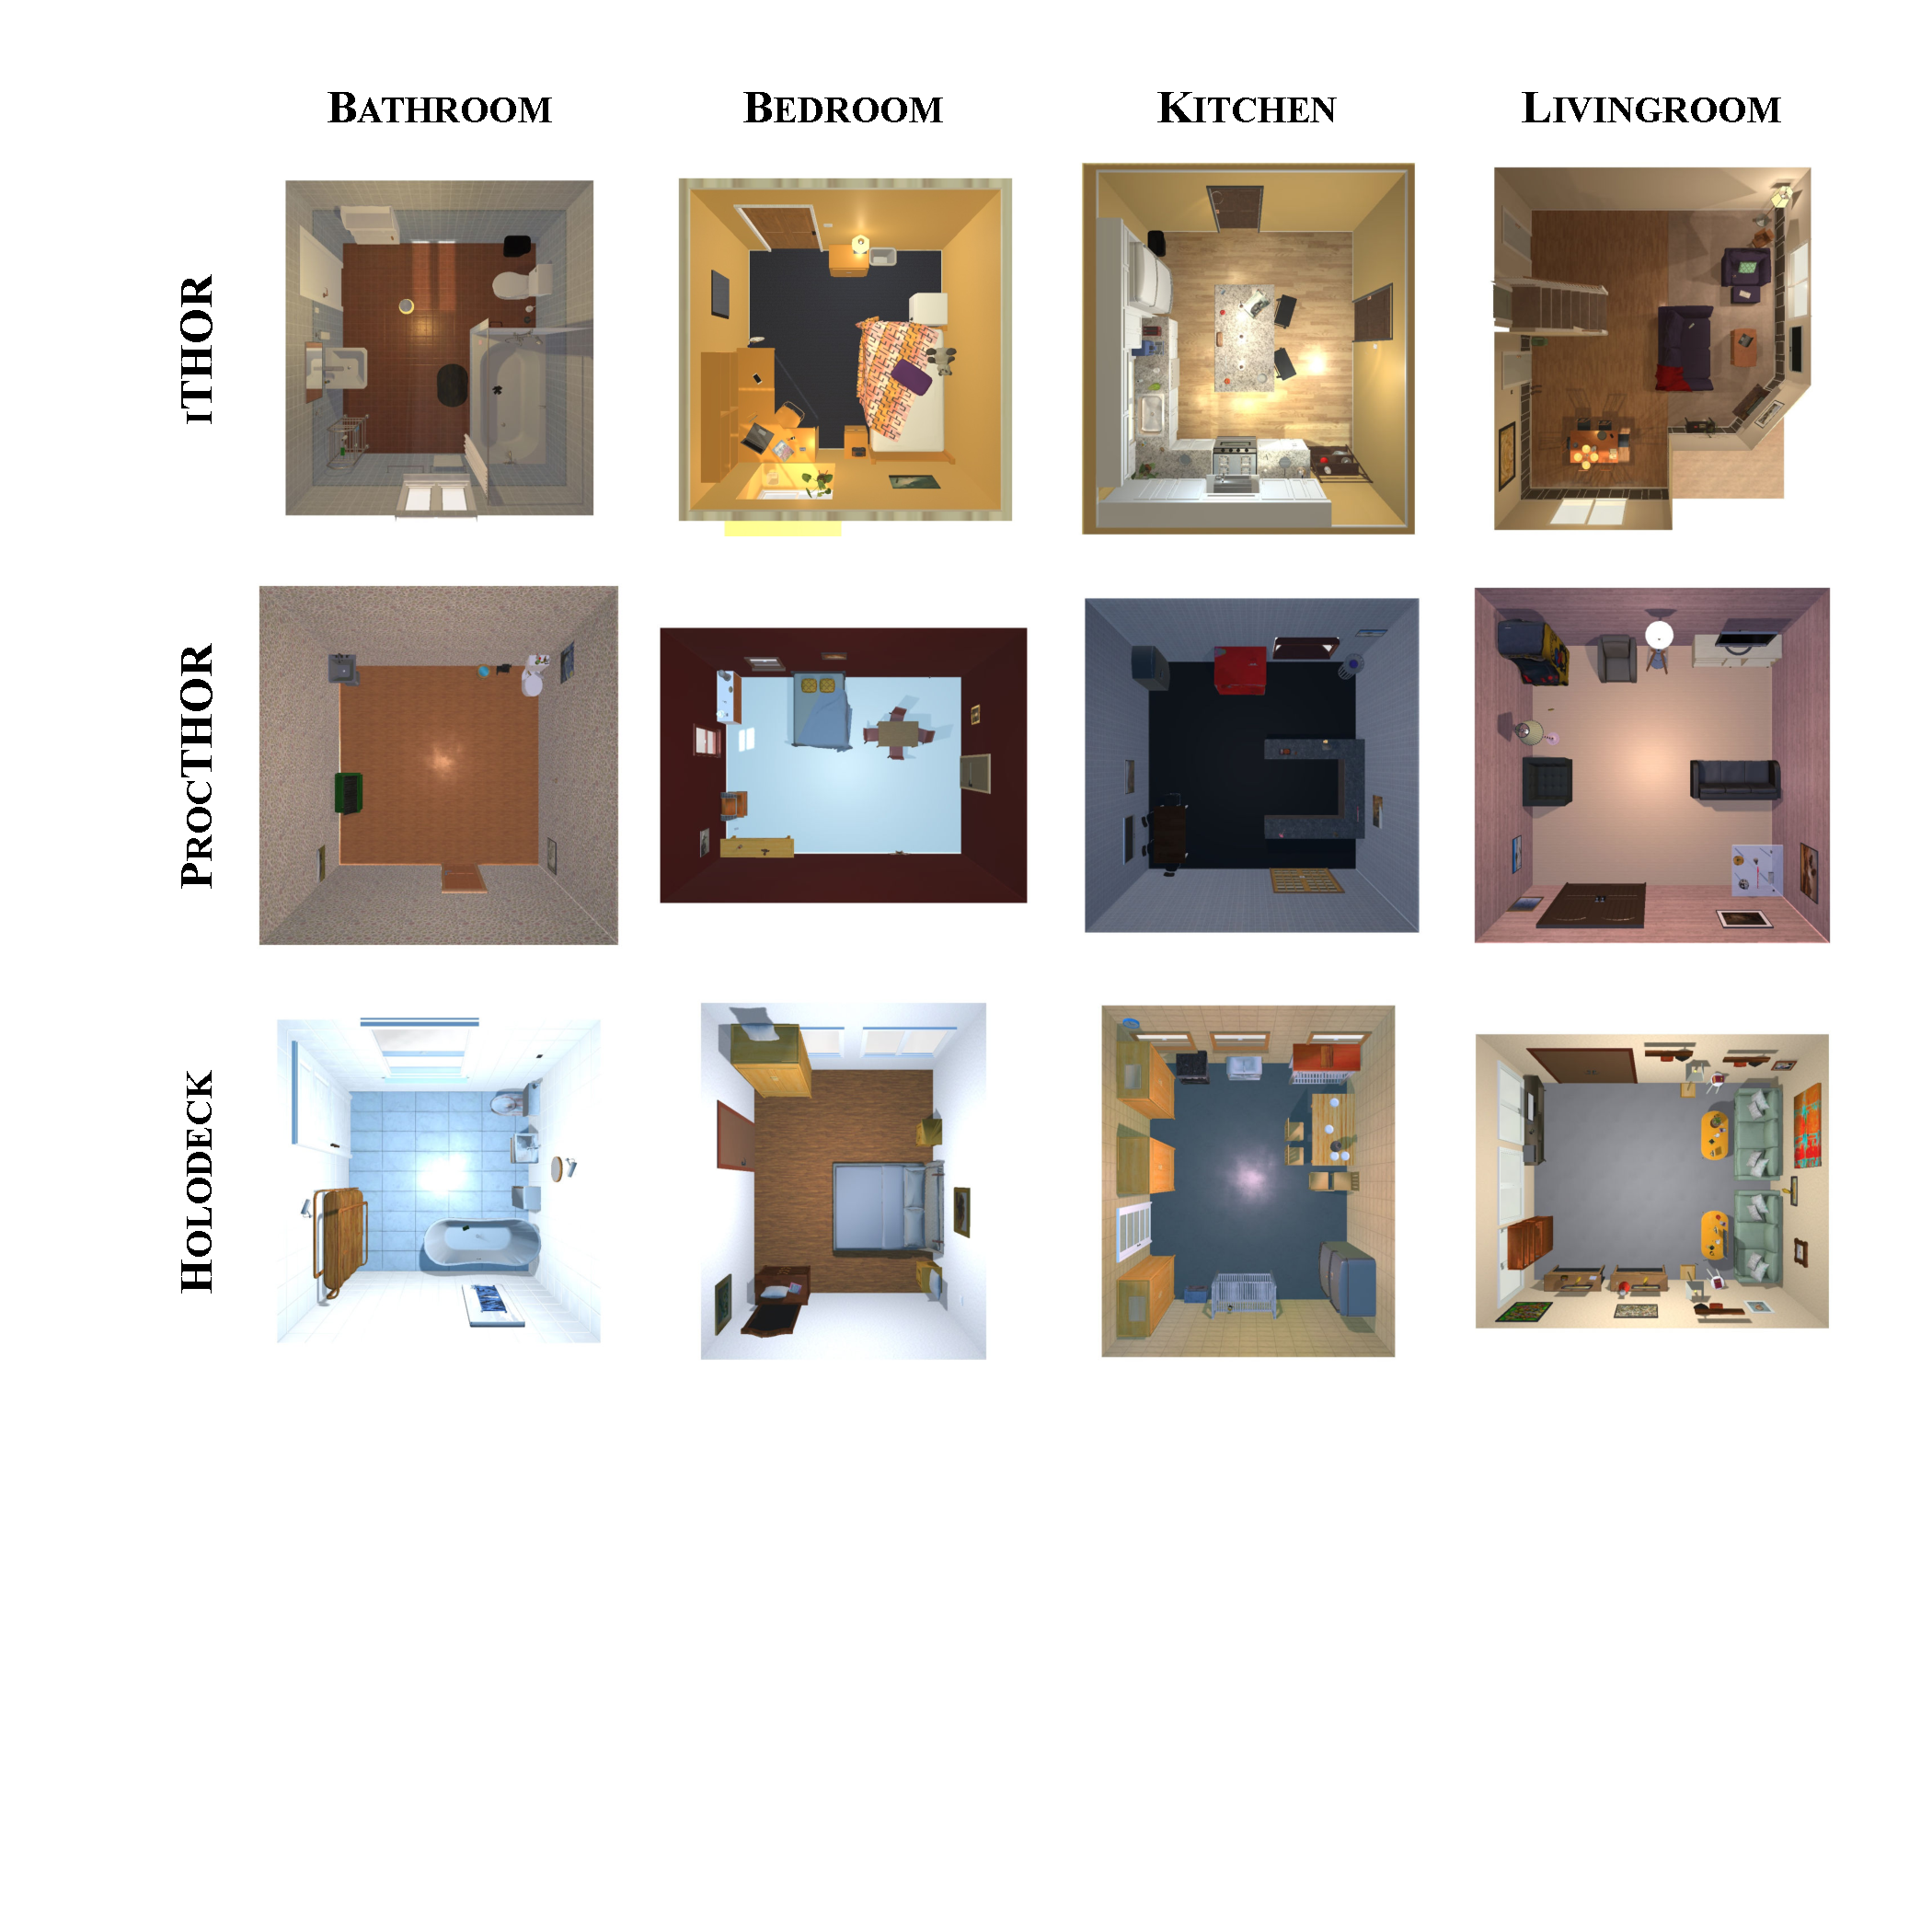
\includegraphics[width=17cm]{images/system_compare.pdf}
    \caption{Qualitative examples on four types of residential scenes from iTHOR, \procthor, and \holodeck.}
    \label{fig: system_compare}
    \vspace{-0.4cm}
\end{figure*}

\begin{figure*}[!b]
\centering
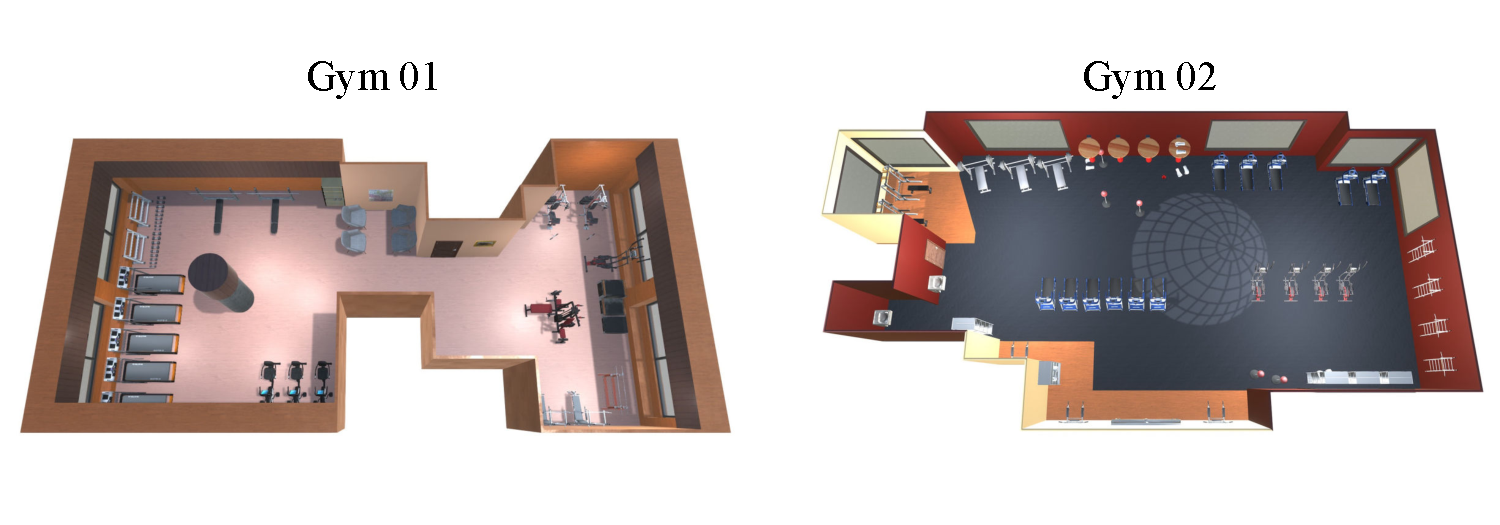
\includegraphics[width=16cm]{images/novelty_thor_continued.pdf}
    \caption{Top-down view of \noveltythor. Each scene type has two instances.}
    \label{fig: noveltythor}
    \vspace{-0.4cm}
\end{figure*}

\begin{figure*}[!t]
\centering
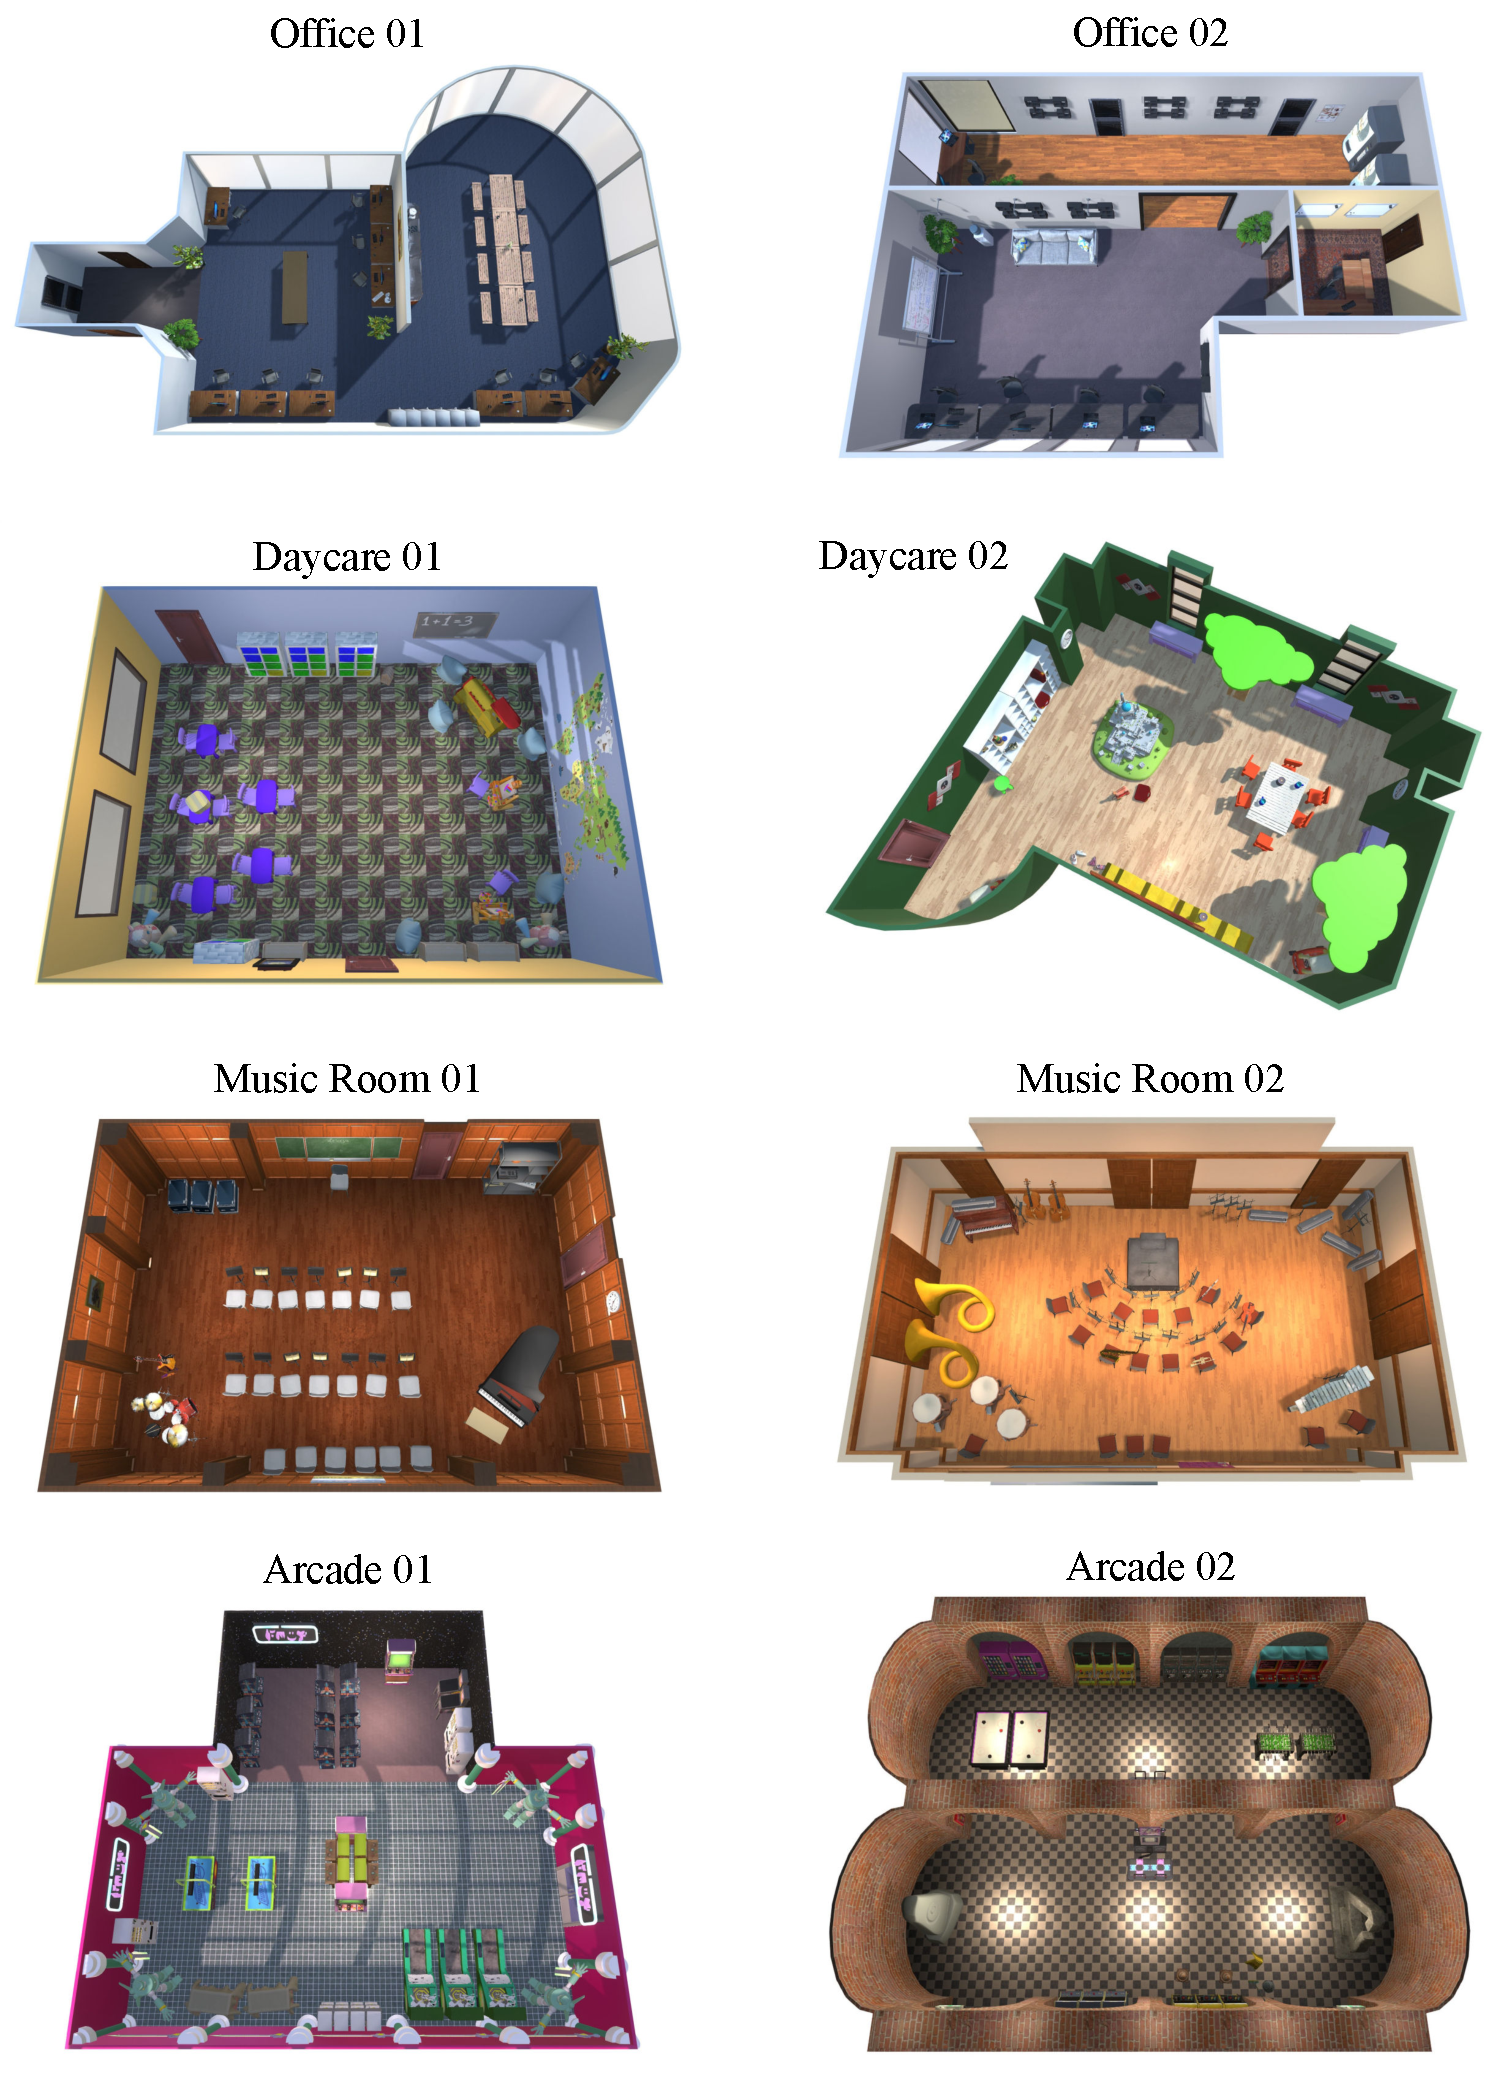
\includegraphics[width=16cm]{images/novelty_thor.pdf}
    \caption{Top-down view of \noveltythor (continued).}
    \label{fig: noveltythor_continued}
    \vspace{-0.4cm}
\end{figure*}